 
\section{Phương trình, bất phương trình mũ và lôgarit}
\subsection{Tóm tắt lý thuyết}
\begin{tomtat}
	\subsubsection{Phương trình mũ}
	\begin{itemize}
		\item Phương trình mũ là phương trình có chứa ẩn ở số mũ của lũy thừa.
		\item Phương trình mũ cơ bản ẩn $x$ có dạng $a^x=b \,\, (a>0, a\neq 1)$.
		\begin{itemize}
			\item Nếu $b\leq 0$ thì phương trình vô nghiệm.
			\item Nếu $b>0$ thì phương trình có nghiệm duy nhất $x=\log_a b$.
		\end{itemize}
	\end{itemize}
	\begin{nx}\hfill
		\begin{itemize}
			\item Với $a>0, a\neq 1, b>0$ thì $a^{f(x)}=b \Leftrightarrow f(x)=\log_a b$.
			\item Với $a>0, a\neq 1$ thì $a^{f(x)}=a^{g(x)} \Leftrightarrow f(x)=g(x)$.\\
			Cách giải phương trình mũ như trên thường được gọi là phương pháp \textbf{\textit{đưa về cùng cơ số}}.
		\end{itemize}
	\end{nx}
	\subsubsection{Phương trình lôgarit}
	\begin{itemize}
		\item Phương trình lôgarit là phương trình có chứa ẩn trong biểu thức dưới dấu lôgarit.
		\item Phương trình lôgarit cơ bản có dạng $\log_a x=b$ ($a>1, a\neq 1$).\\
		Phương trình đó có một nghiệm là $x=a^b$.
	\end{itemize}
	\begin{nx}\hfill
		\begin{itemize}
			\item Với $a>0, a\neq 1$ thì $\log_a f(x)=b \Leftrightarrow f(x)=a^b$.
			\item Cho $a>0, a\neq 1$. Ta có: $\log_a f(x)=\log_a g(x) \Leftrightarrow \heva{&f(x)>0\\&f(x)=g(x).}$
		\end{itemize}
	\end{nx}
	\subsubsection{Bất phương trình mũ}
	\begin{itemize}
		\item Bất phương trình mũ là bất phương trình có chứa ẩn ở số mũ của lũy thừa.
		\item Bất phương trình mũ cơ bản là bất phương trình có một trong những dạng sau:
		$$a^x>b; a^x<b; a^x\geq b; a^x \leq b\,\, (a>0,a\neq 1).$$
		\item Xét bất phương trình mũ: $a^x>b\, \, (a>0, a\neq 1)$.
		\begin{itemize}
			\item Nếu $b\leq 0$, tập nghiệm của bất phương trình đã cho là $\mathbb{R}$ (vì $a^x>0\geq b, \forall x\in \mathbb{R}$).
			\item Nếu $b>0$ thì bất phương trình tương đương với $a^x>a^{\log_a^b}$.\\
			Với $a>1$, nghiệm của bất phương trình là $x>\log_a b$.\\
			Với $0<a<1$, nghiệm của bất phương trình là $x<\log_a b$.
		\end{itemize}
	\end{itemize}
	\begin{nx}
		Các bất phương trình mũ cơ bản còn lại được giải tương tự.
	\end{nx}
	\subsubsection{Bất phương trình lôgarit}
	\begin{itemize}
		\item Bất phương trình lôgarit là bất phương trình có chứa ẩn trong biểu thức dưới dấu lôgarit
		\item Bất phương trình lôgarit cơ bản là bất phương trình lôgarit có một trong các dạng sau:
		$$\log_a x>b; \log_a x<b;\log_a x\geq b; \log_a x\leq b\, (a>0, a\neq 1).$$
		\item Xét bất phương trình $\log_ax>b$ ($a>0, a\neq 1$).\\
		Bất phương trình tương đương với $\log_a x>\log_a a^b$.
		\begin{itemize}
			\item Với $a>1$, nghiệm của bất phương trình là $x>a^b$.
			\item Với $0<a<1$, nghiệm của bất phương trình là $0<x<a^b$.
		\end{itemize}
	\end{itemize}
	\begin{nx}
		Các bất phương trình lôgarit cơ bản còn lại được giải tương tự.
	\end{nx}
\end{tomtat} \setcounter{subsubsection}{0}
\setcounter{ex}{0}
\setcounter{bt}{0}
\subsection{Các dạng toán thường gặp}
\begin{dang}{Phương trình mũ, lôgarit cơ bản}
	Sử dụng các công thức
	\begin{itemize}
		\item $a^{f(x)}=b \Leftrightarrow f(x)=\log_a b$ $(a,b>0; a\neq 1)$.
		\item $\log_a f(x)=b\Leftrightarrow f(x)=a^b$ $(a>0;a\neq 1)$.
	\end{itemize}
\end{dang}
\subsubsection{Ví dụ minh hoạ}

\begin{vd}%[1C6B4-1]
	Tìm điều kiện xác định của các phương trình sau
	\begin{listEX}[2]
		\item $\log_2(2x-1)=3$.
		\item $\log_3\left(-x^2+2x\right)=-1$.
	\end{listEX}
	\loigiai{
		\begin{enumerate}
			\item Điều kiện $2x-1>0\Leftrightarrow x>\dfrac{1}{2}$.
			\item Điều kiện $-x^2+2x>0\Leftrightarrow 0<x<2$.
		\end{enumerate}
	}
\end{vd}

\begin{vd} %[1C6B4-2]
	Giải mỗi phương trình sau:
	\begin{listEX}[2]
		\item $4^{2x-3}=5$;
		\item $10^{x+1}-2\cdot 10^x=8$.
	\end{listEX}
	\loigiai{
		Ta có 
		\begin{enumerate}
			\item $4^{2x-3}=5 \Leftrightarrow 2x-3=\log_4 5  \Leftrightarrow 2x=3+\log_4 5 \Leftrightarrow 
			x = \dfrac{1}{2}\left(3+\log_4 5\right)$.\\
			Vậy phương trình có nghiệm là $x=\dfrac{1}{2}\left(3+\log_4 5\right)$.
			\item $10^{x+1}-2\cdot 10^x =8 \Leftrightarrow 10\cdot 10^ x-2\cdot 10^x =8 \Leftrightarrow 8\cdot 10^x =8 \Leftrightarrow 10^x =1 \Leftrightarrow x=\log 1 \Leftrightarrow x=0$.\\
			Vậy phương trình có nghiệm là $x=0$.
		\end{enumerate}
	}
\end{vd}

\begin{vd} %[1K6B4-2]
	Giải phương trình $10^{x-1}=2022$.
	\loigiai{
		Lấy lôgarit thập phân hai vế của phương trình ta được $x-1=\log 2022$ hay $x=1+\log 2022$ \\
		Vậy phương trình đã cho có nghiệm duy nhất $x=1+\log 2022$.
	}
\end{vd}

\begin{vd} %[1T6B4-2]
	Giải các phương trình sau
	\begin{listEX}[2]
		\item $2^x=\dfrac{1}{8}$.
		\item $5\cdot 10^x=1$.
		\item $3^{x+2}=\sqrt[3]{9}$.
		\item $2\cdot 10^{2 x}=30$.
	\end{listEX}
	\loigiai{
		\begin{enumerate}
			\item $2^x=\dfrac{1}{8} \Leftrightarrow 2^x=2^{-3} \Leftrightarrow x=-3$.
			\item $5 \cdot 10^x=1 \Leftrightarrow 10^x=\dfrac{1}{5} \Leftrightarrow x=\log \dfrac{1}{5}=-\log 5$.
			\item $3^{x+2}=\sqrt[3]{9}\Leftrightarrow x+2=\dfrac{2}{3}\Leftrightarrow x=-\dfrac{4}{3}$.
			\item $2\cdot 10^{2 x}=30\Leftrightarrow x=\dfrac{1}{2}\log_{10} 15$.
		\end{enumerate}
	}
\end{vd}

\begin{vd} %[1C6B4-2]
	Giải mỗi phương trình sau:
	\begin{listEX}[2]
		\item $\log_2 x=5$;
		\item $\log_4 (5x-4)=2$.
	\end{listEX}	
	\loigiai{
		\begin{enumerate}
			\item Ta có $\log_2 x=5\Leftrightarrow x=2^5 \Leftrightarrow x=32$.\\
			Vậy phương trình có nghiệm là $x=32$.
			\item Ta có $\log_4 (5x-4)=2 \Leftrightarrow 5x-4=4^2 \Leftrightarrow 5x=20 \Leftrightarrow x=4$.\\
			Vậy phương trình có nghiệm là $x=4$.
		\end{enumerate}
	}
\end{vd}

\begin{vd} %[1K6B4-2]
	Giải phương trình $4+3\log(2x)=16$.
	\loigiai{
		Điều kiện $2x>0$ hay $x>0$.\\
		Phương trình trở thành $\log(2x)=4$. \\
		Từ đó $2x=10^4$ hay $x=5000$ (thỏa mãn điều kiện).\\
		Vậy phương trình đã cho có nghiệm là  $x=5000$.
	}
\end{vd}

\begin{vd} %[1T6B4-2]
	Giải các phương trình sau
	\begin{listEX}[2]
		\item $\log _3 x=-2$.
		\item $\log _{\tfrac{1}{2}}(x-2)=-2$.
	\end{listEX}
	\loigiai{
		\begin{enumerate}
			\item Điều kiện: $x>0$.\\
			$\log_3 x=-2 \Leftrightarrow x=3^{-2}=\dfrac{1}{3^2}=\dfrac{1}{9}$.
			\item Điều kiện: $x>2$.\\
			$\log _{\tfrac{1}{2}}(x-2)=-2\Leftrightarrow x-2=4\Leftrightarrow x=6$.
		\end{enumerate}
	}
\end{vd}

\subsubsection{Bài tập rèn luyện} 

\begin{bt}
	Tìm điều kiện xác định của các phương trình sau
	\begin{listEX}[2]
		\item $\log_5(3-4x)=2$.
		\item $\log(x^2-2x-3)=3$.
	\end{listEX}
	\loigiai{
		\begin{enumerate}
			\item Điều kiện $3-4x>0\Leftrightarrow x<\dfrac{3}{4}$.
			\item Điều kiện $x^2-2x-3>0\Leftrightarrow \hoac{&x>3\\&x<-1}$.
		\end{enumerate}
	}
\end{bt}

\begin{bt}
	Giải các phương trình sau
	\begin{listEX}[2]		
		\item $(0{,}3)^{x-3}=1$.
		\item $3^{x-1}=27$.
		\item $5^{3x-2}=25$.
		\item  $3^{x+2}=7$.
		\item $3\cdot 10^{2x+1}=5$.
		\item $10^{1-2x}=100000$.
	\end{listEX}
	\loigiai{
		\begin{enumerate}
			\item  Ta có $(0{,}3)^{x-3}=1 \Leftrightarrow x-3=\log_{0{,}3} 1\Leftrightarrow x-3=0 \Leftrightarrow x=3$.\\
			Vậy phương trình có nghiệm là $x=3$.
			\item Ta có $3^{x-1}=27\Leftrightarrow3^{x-1}=3^3\Leftrightarrow x-1=3\Leftrightarrow x=4$.\\\\
			Vậy phương trình có nghiệm là $x=4$.
			\item  Ta có $5^{3x-2}=25 \Leftrightarrow 3x-2=\log_5 25 \Leftrightarrow 3x-2=2 \Leftrightarrow 3x=4 \Leftrightarrow x=\dfrac{4}{3}$.\\
			Vậy phương trình có nghiệm là $x=\dfrac{4}{3}$.
			\item  $3^{x+2}=7\Leftrightarrow x+2=\log_37\Leftrightarrow  x=\log_3 7 -2$.\\
			Vậy phương trình có nghiệm là $x=\log_37-2$.
			\item $3\cdot 10^{2x+1}=5\Leftrightarrow 2x+1=\log \dfrac{5}{3}\Leftrightarrow x=\dfrac{1}{2}\left(\log \dfrac{5}{3}-1\right)$.\\
			Vậy phương trình có nghiệm là $x=\dfrac{1}{2}\left(\log \dfrac{5}{3}-1\right)$.
			\item $10^{1-2x}=100000\Leftrightarrow 10^{1-2x}=10^5\Leftrightarrow 1-2x=5\Leftrightarrow x=-2$.\\
			Vậy phương trình có nghiệm là $x=-2$.
		\end{enumerate}
	}
\end{bt}

\begin{bt}
	Giải các phương trình sau
	\begin{listEX}[2]
		\item $\log (x+1)=2$.
		\item $\log _6(4 x+4)=2$.
		\item $\log_{\frac{1}{2}} (x+1)=-3$.	
		\item $\log _3 x+\log _3(x-2)=1$.
	\end{listEX}
	\loigiai{
		\begin{enumerate}
			\item Ta có $\log (x+1)=2\Leftrightarrow x+1=10^2\Leftrightarrow x=99$.\\
			Vậy phương trình có nghiệm là $x=99$.
			\item Ta có $\log_6 (4x+4)=2\Leftrightarrow 4x+4=6^2\Leftrightarrow x=8$.\\
			Vậy phương trình có nghiệm là $x=8$.
			\item Ta có $\log_{\tfrac{1}{2}} (x+1)=-3 \Leftrightarrow x+1=\left(\dfrac{1}{2}\right)^{-3} \Leftrightarrow x+1=8 \Leftrightarrow x=7$.\\
			Vậy phương trình có nghiệm là $x=7$.		
			\item Điều kiện $x>2$.\\
			Ta có $\log_3 x+\log_3(x-2)=1\Leftrightarrow \log_3 \left[x(x-2)\right]=1\Leftrightarrow x^2-2x=3\Leftrightarrow \hoac{&x=-1 \text{ (loại)}\\&x=3 \text{ (thỏa mãn).}}$\\
			Vậy phương trình có nghiệm là $x=3$.
		\end{enumerate}
	}
\end{bt}

\subsubsection{Bài tập trắc nghiệm}
\Opensolutionfile{ans}[ANS/ans-1-6-4-2]
\begin{ex}
	Điều kiện xác định của phương trình $\log_3(x-2)=1$ là
	\choice
	{$x=2$}
	{$x\geq 2$}
	{\True $x>2$}
	{$x>5$}
\end{ex}

\begin{ex}
	Điều kiện xác định của phương trình $\ln \dfrac{1-x}{x+1}=3$ là
	\choice
	{$x<1$}
	{$x\neq -1$}
	{$x<-1$ hoặc $x>1$}
	{\True $-1<x<1$}
\end{ex}

\begin{ex}
	Tìm nghiệm của phương trình $3^{x-1}=27$.
	\choice
	{$x=9$}
	{$x=3$}
	{\True $x=4$}
	{$x=10$}
	\loigiai{
		Ta có
		\[3^{x-1}=27\Leftrightarrow 3^{x-1}=3^3\Leftrightarrow x-1=3\Leftrightarrow x=4.\]
	}
\end{ex}

\begin{ex}
	Tập nghiệm của phương trình $3^{2x^2-x}=3$ là
	\choice
	{$\left\{ 0;2\right\}$}
	{$\left\{ 0;\dfrac{1}{2}\right\}$}
	{$\left\{-1;\dfrac{1}{2}\right\}$}
	{\True $\left\{-\dfrac{1}{2};1\right\}$}
	\loigiai{
		Ta có $3^{2x^2-x}=3\Leftrightarrow 2x^2-x=1\Leftrightarrow \hoac{&x=1\\&x=-\dfrac{1}{2}.}$
	}
\end{ex}

\begin{ex}
	Tập nghiệm của phương trình $\log_2(x^2-1)=3$ là
	\choice
	{\True $\{-3;3\}$}
	{$\{-3\}$}
	{$\{3\}$}
	{$\left\{-\sqrt{10};\sqrt{10}\right\}$}
	\loigiai{
		Ta có $\log_2(x^2-1)=3 \Leftrightarrow x^2-1=2^3\Leftrightarrow \hoac{&x=3\\&x=-3.}$\\
		Vậy tập nghiệm của phương trình đã cho là $ \lbrace -3; 3\rbrace $.
	}
\end{ex}


\begin{ex}
	Tập nghiệm của phương trình $\log(10x)=2$ là
	\choice
	{$\left\{\dfrac{1}{10}\right\}$}
	{\True $\{10\}$}
	{$\{1\}$}
	{$\{100\}$}
	\loigiai{
		Ta có $\log (10 x)=2 \Leftrightarrow 10x=10^2 \Leftrightarrow x=10$.\\
		Vậy phương trình đã cho có tập nghiệm $\{10\}$.
	}
\end{ex}

\begin{ex}
	Gọi $x_1$, $x_2$ là hai nghiệm của phương trình $2^{x^2-3x+2}=1$. Tính $P=x_1^2+x_2^2$.
	\choice
	{$P=10$}
	{$P=8$}
	{\True $P=5$}
	{$P=13$}
	\loigiai{
		Ta có $2^{x^2-3x+2}=1\Leftrightarrow x^2+3x+2=0\Leftrightarrow \hoac{&x=-1\\&x=-2}\Rightarrow P=x_1^2+x_2^2=5$.}
\end{ex}

\begin{ex}
	Tìm tập nghiệm $S$ của phương trình $\log_2(x-1)+\log_2(x+1)=3$.
	\choice
	{$S=\{-3;3\}$}
	{$S=\{4\}$}
	{\True $S=\{3\}$}
	{$S=\{-\sqrt{10};\sqrt{10}\}$}
	\loigiai{
		Từ điều kiện $x>1$ ta loại được các phương án $S=\{-3;3\}$ và $S=\{-\sqrt{10};\sqrt{10}\}$. Thay $x=4$ vào phương trình không thỏa mãn nên loại phương án $S=\{4\}$.
	}
\end{ex}


\begin{ex}
	Phương trình $2^x+2^{x-1}+2^{x-2}=3^x-3^{x-1}+3^{x-2}$ có nghiệm
	\choice
	{$x=5$}
	{\True $x=2$}
	{$x=4$}
	{$x=3$}
	\loigiai{
		Ta có $\begin{aligned}[t]
			2^x+2^{x-1}+2^{x-2}=3^x-3^{x-1}+3^{x-2} & \Leftrightarrow 2^x+\dfrac{1}{2} \cdot 2^x+\dfrac{1}{4} \cdot 2^x=3^x-\dfrac{1}{3} \cdot 3^x+\dfrac{1}{9} \cdot 3^x \\
			&\Leftrightarrow \dfrac{7}{4} \cdot 2^x=\dfrac{7}{9} \cdot 3^x \\
			&\Leftrightarrow \left(\dfrac{2}{3}\right)^x=\dfrac{4}{9} \Leftrightarrow x=2.
		\end{aligned}$ \\
		Vậy phương trình có nghiệm là $x=2$.
	}
\end{ex}


\begin{ex}
	Biết rằng phương trình $\log_2x+\log_3x=1+\log_2x\log_3x$ có hai nghiệm $x_1$, $x_2$. Giá trị của $x_1^2+x_2^2$ bằng
	\choice
	{$5$}
	{$25$}
	{$2$}
	{\True $13$}
	\loigiai{
		Ta có phương trình tương đương	
		\begin{eqnarray*}
			\log_2x \left(1-\log_3x\right)-\left(1-\log_3x\right)=0
			&\Leftrightarrow& \left(\log_2x-1\right) \cdot \left(1-\log_3x\right)=0\\
			&\Leftrightarrow &\hoac{&\log_2x=1\\&\log_3x=1}\\
			&\Leftrightarrow&\hoac{&x_1=2\\&x_2=3.}
		\end{eqnarray*}
		Vậy $x_1^2+x_2^2=13$.
	}
\end{ex}


\begin{ex}
	Tổng tất cả các nghiệm của phương trình $ 2^{x^2-2x-1}\cdot 3^{x^2-2x}=18 $ bằng
	\choice
	{$ 1 $}
	{$ -2 $}
	{\True $ 2 $}
	{$ -1 $}
	\loigiai{
		Ta có $ 2^{x^2-2x-1}\cdot 3^{x^2-2x}=18\Leftrightarrow 2^{x^2-2x}\cdot\dfrac{1}{2}\cdot 3^{x^2-2x}=18\Leftrightarrow 6^{x^2-2x}=36\Leftrightarrow x^2-2x=2\Leftrightarrow x=1\pm \sqrt{3} $.\\
		Tổng các nghiệm của phương trình là $ \left(1+\sqrt{3}\right)+\left(1-\sqrt{3}\right)=2 $.
	}
\end{ex}


\begin{ex}
	Tổng tất cả các nghiệm của phương trình $\log_{ 2 } \left |x^2+2x-3 \right |-\log_{ 2 } \left |x+3 \right |=3$ bằng
	\choice
	{$9$}
	{$-2$}
	{$-4$}
	{\True $2$}
	\loigiai{
		Điều kiện $x\ne -3$ và $x\ne 1$. Khi đó phương trình đã cho tương đương với
		\[\log_2\left |\dfrac{x^2+2x-3}{x+3} \right | =3\Leftrightarrow \log_2\left |x-1 \right |=3\Leftrightarrow \left |x-1 \right |=9\Leftrightarrow \hoac{&x=10\\&x=-8}\quad \text{(thỏa mãn)}.\]
		Vậy, tổng các nghiệm của phương trình đã cho bằng $2$.
	}
\end{ex}
\Closesolutionfile{ans}
\begin{indapan}{10}
	{ANS/ans-1-6-4-2}
\end{indapan}

\begin{dang}{Bất phương trình mũ, lôgarít cơ bản}
	Xét bất phương trình mũ: $a^x>b\, \, (a>0, a\neq 1)$.
	\begin{itemize}
		\item[•] Nếu $b\leq 0$, tập nghiệm của bất phương trình đã cho là $\mathbb{R}$ (vì $a^x>0\geq b, \forall x\in \mathbb{R}$).
		\item[•] Nếu $b>0$ thì bất phương trình tương đương với $a^x>a^{\log_a^b}$.\\
		Với $a>1$, nghiệm của bất phương trình là $x>\log_a b$.\\
		Với $0<a<1$, nghiệm của bất phương trình là $x<\log_a b$.		
	\end{itemize}
	Bất phương trình tương đương với $\log_a x>\log_a a^b$.
	\begin{itemize}
		\item[•] Với $a>1$, nghiệm của bất phương trình là $x>a^b$.
		\item[•] Với $0<a<1$, nghiệm của bất phương trình là $0<x<a^b$.
	\end{itemize}
\end{dang}
\subsubsection{Ví dụ minh hoạ}
\begin{vd} %[1C6B4-3]
	Giải mỗi bất phương trình sau:
	\begin{listEX}[2]
		\item $5^x>12$;
		\item $(0{,}3)^{x+1}>1{,}7$.
	\end{listEX}
	\loigiai{
		Ta có:
		\begin{enumerate}
			\item $5^x>12\Leftrightarrow x>\log_5 12$.\\
			Vậy tập nghiệm của bất phương trình là $(\log_5 12;+\infty)$.
			\item $(0{,}3)^{x+1}>1{,}7 \Leftrightarrow x+1<\log_{0{,}3} 1{,}7 \Leftrightarrow x<-1+\log_{0{,}3} 1{,}7$.\\
			Vậy tập nghiệm của bất phương trình là $(-\infty;-1+\log_{0{,}3} 1{,}7)$.	
		\end{enumerate}
	}
\end{vd}
\begin{vd} %[1K6YK-5]
	Giải bất phương trình $16^{x}>\dfrac{1}{8}$.
	\loigiai{
		Ta có $16^{x}>\dfrac{1}{8}\Leftrightarrow 2^{4x}>2^{-3}\Leftrightarrow 4x>-3\Leftrightarrow x>-\dfrac{3}{4}$.
	}
\end{vd}
\begin{vd} %[1C6B4-3]
	Giải mỗi bất phương trình sau
	\begin{listEX}[2]
		\item $\log_{\frac{1}{2}}x>-2$;
		\item $\log_2(x+1)>3$.
	\end{listEX}
	\loigiai{
		Ta có
		\begin{enumerate} 
			\item $\log_{\frac{1}{2}}x>-2 \Leftrightarrow 0<x<\left(\dfrac{1}{2}\right)^{-2} \Leftrightarrow 0<x<2^2 \Leftrightarrow 0<x<4$.\\
			Vậy tập nghiệm của bất phương trình là $(0;4)$.
			\item $\log_2(x+1)>3 \Leftrightarrow x+1>2^3 \Leftrightarrow x>7$.\\
			Vậy tập nghiệm của bất phương trình là $(7;+\infty)$.
		\end{enumerate}
	}
\end{vd}
\begin{vd} %[1T6Y4-3]
	Giải các bất phương trình sau
	\begin{listEX}[3]
		\item $10^x<0{,}001$.
		\item $0{,}4^x>2$.
		\item $\left(\dfrac{1}{2}\right)^x \geq 2 \cdot 4^{2x}$.
	\end{listEX}
	\loigiai{
		\begin{enumerate}
			\item $10^x<0{,}001 \Leftrightarrow 10^x<10^{-3} \Leftrightarrow x<-3$ (do $10>1$ ).
			\item $0{,}4^x>2 \Leftrightarrow x<\log _{0{,}4} 2$ (do $0<0{,}4<1)$.
			\item
			\allowdisplaybreaks
			\begin{eqnarray*}
				&&\left(\dfrac{1}{2}\right)^x \geq 2 \cdot 4^{2 x}  \Leftrightarrow\left(2^{-1}\right)^x \geq 2 \cdot\left(2^2\right)^{2 x} \Leftrightarrow 2^x \geq 2^{1+4 x} \\
				&\Leftrightarrow&-x \geq 1+4 x \Leftrightarrow 5 x \leq-1 \Leftrightarrow x \leq-\dfrac{1}{5}.
			\end{eqnarray*}
		\end{enumerate}
	}
\end{vd}
\begin{vd} %[1T6Y4-3]
	Giải các bất phương trình sau
	\begin{listEX}[2]
		\item $\log _{\tfrac{1}{3}}(x+1)<2$.
		\item $\log _5(x+2) \leq 1$.
	\end{listEX}
	\loigiai{
		\begin{enumerate}
			\item Điều kiện: $x>-1$.\\
			$\log _{\tfrac{1}{3}}(x+1)<2\Leftrightarrow x+1>\left(\dfrac{1}{3}\right)^2\Leftrightarrow x>-\dfrac{8}{9}$.\\
			Vậy nghiệm của bất phương trình là $x>-\dfrac{8}{9}$
			\item Điều kiện $x>-2$.\\
			$\log _5(x+2) \leq 1\Leftrightarrow x+2\le 5\Leftrightarrow x\le 3$.\\
			Vậy nghiệm của bất phương trình là $-2<x\le 3$.
	\end{enumerate}}
\end{vd}
\subsubsection{Bài tập rèn luyện} 
\begin{bt}
	Giải mỗi bất phương trình sau
	\begin{listEX}[2]
		\item $3^x>\dfrac{1}{243}$.
		\item $\log (x-1)<0$.		
	\end{listEX}
	\loigiai{
		Ta có
		\begin{enumerate}
			\item  $3^x>\dfrac{1}{243} \Leftrightarrow x>\log_3 \dfrac{1}{243} \Leftrightarrow x>-5$.\\
			Vậy tập nghiệm của bất phương trình là $(-5;+\infty)$.
			\item   $\log (x-1)<0 \Leftrightarrow \heva{&x-1>0\\&x-1<10^0} 
			\Leftrightarrow \heva{&x>1\\&x<2} \Leftrightarrow 1<x<2$.\\
			Vậy tập nghiệm của bất phương trình là $(1;2)$.
		\end{enumerate}
	}
\end{bt}
\begin{bt}
	Giải các bất phương trình sau
	\begin{listEX}[2]
		\item $\left(\dfrac{1}{3}\right)^{2x+1} \leqslant 9$.
		\item $4^x>2^{x-2}$.
	\end{listEX}
	\loigiai{
		\begin{enumerate}
			\item $\left(\dfrac{1}{3}\right)^{2x+1} \leqslant 9\Leftrightarrow 2x+1\geqslant -2\Leftrightarrow x\geqslant -\dfrac{3}{2}$.
			\item $4^x>2^{x-2}\Leftrightarrow 2^{2x}>2^{x-2}\Leftrightarrow 2x>x-2\Leftrightarrow x>-2$.
		\end{enumerate}	
	}
\end{bt}
\begin{bt}
	Giải các bất phương trình sau
	\begin{listEX}[2]
		\item $\log_2(x-2)<2$.
		\item $\log (x+1) \geq \log (2x-1)$.
	\end{listEX}
	\loigiai{
		\begin{enumerate}
			\item Điều kiện $x>2$.
			$$\log_2(x-2)<2\Leftrightarrow x-2<4\Leftrightarrow x<6.$$
			Kết hợp điều kiện ta có nghiệm của bất phương trình là $2<x<6$.
			\item Điều kiện $x>\dfrac{1}{2}$.
			$$\log (x+1) \geqslant \log (2x-1)\Leftrightarrow x+1\geqslant 2x-1\Leftrightarrow x\leqslant 2.$$
			Kết hợp với điều kiện, ta có nghiệm của bất phương trình là $\dfrac{1}{2}<x\leqslant 2$.
		\end{enumerate}
	}
\end{bt}
\subsubsection{Bài tập trắc nghiệm}
\Opensolutionfile{ans}[ANS/ans-1-6-4-3]
\begin{ex}
	Tìm tập nghiệm của bất phương trình $\left(\dfrac{1}{2}\right)^x<4$.
	\choice
	{\True $(-2;+\infty)$}
	{$(0;4)$}
	{$(-\infty;-2)$}
	{$(-\infty;2)$}
	\loigiai{
		Ta có $\left(\dfrac{1}{2}\right)^x<4\Leftrightarrow x>\log_{\frac{1}{2}}4=-2$.\\
		Vậy tập nghiệm của bất phương trình là $(-2;+\infty)$.
	}
\end{ex}

\begin{ex}
	Giải bất phương trình $3^{x+2}\ge \dfrac{1}{9}$.
	\choice
	{$x>0$}
	{\True $x\ge -4$}
	{$x<4$}
	{$x<0$}
	\loigiai{
		Ta có $3^{x+2}\ge \dfrac{1}{9}\Leftrightarrow3^{x+2}\ge 3^{-2}\Leftrightarrow x+2\ge -2\Leftrightarrow x\ge -4$.}
\end{ex}
\begin{ex}
	Tập nghiệm của bất phương trình $\log _{2}(x-1)>3$ là
	\choice
	{$(4 ;+\infty)$}
	{\True $(9 ;+\infty)$}
	{$(10 ;+\infty)$}
	{$(1 ;+\infty)$}
	\loigiai{
		Ta có    $\log _{2}(x-1)>3 \Leftrightarrow x-1 > 8 \Leftrightarrow x >9$. \\
		Vậy tập nghiệm của bất phương trình là $(9 ;+\infty)$.
	}
\end{ex}
\begin{ex}
	Tập nghiệm của bất phương trình $\log_3x\le 1$ là
	\choice
	{$(-\infty;3]$}
	{$(-\infty;1]$}
	{\True $(0;3]$}
	{$(0;1]$}
	\loigiai{
		Ta có $\log_3x\le 1\Leftrightarrow \heva{&x>0\\&x\le 3. }$\\
		Vậy tập nghiệm của bất phương trình $\log_3x\le 1$ là $(0;3]$.
	}
\end{ex}
\begin{ex}
	Tìm tập nghiệm $S$ của bất phương trình $\log_2(2x+1) \geq \log_2(x-1)$.
	\choice
	{$S=[2;+\infty)$}
	{$S=[-2;+\infty)$}
	{$S=\mathbb{R}$}
	{\True $S=(1;+\infty)$}
	\loigiai
	{
		Ta có
		\begin{eqnarray*}
			& & \log_2(2x+1) \geq \log_2(x-1) \Leftrightarrow \heva{ &x-1 > 0 \\ &2x+1 \geq x-1} \Leftrightarrow \heva{& x>1 \\ &x \geq -2 } \Leftrightarrow x>1.
		\end{eqnarray*}
		Vậy tập nghiệm của bất phương trình đã cho là $S = (1;+\infty)$.
	}
\end{ex}

\begin{ex}
	Tập nghiệm của bất phương trình $\left(\dfrac{1}{2}\right)^{\sqrt{x}}<\dfrac{1}{2}$ là
	\choice
	{$(-\infty;1)$}
	{$(0;1)$}
	{\True $(1;+\infty)$}
	{$\mathbb{R}$}
	\loigiai{
		Điều kiện $x\geq 0$.\\
		Với điều kiện trên, bất phương trình đã cho tương đương với $\sqrt{x} > 1 \Leftrightarrow x > 1$.\\
		Vậy tập nghiệm là $(1;+\infty)$.
	}
\end{ex}
\begin{ex}
	Tập nghiệm của bất phương trình ${{\log }_2}\left( 3-x \right)<2$ là
	\choice
	{$\left( 1;3 \right)$}
	{$\left( 3;+\infty \right)$}
	{$\left( -\infty ;1 \right)$}
	{\True $\left( -1;3 \right)$}
	\loigiai{
		Điều kiện: $3-x>0 \Leftrightarrow x<3$.\\
		Ta có
		$$\log _{2}(3-x)<2 \Leftrightarrow 3-x<2^2 \Leftrightarrow x>-1.$$
		Kết hợp điều kiện ta có tập nghiệm của bất phương trình là $S=(-1;3)$.
	}
\end{ex}
\begin{ex}%Câu 21%[PTD, Tex hóa Nhóm WTB, 2020]%[Nguyễn Việt Long]%[2D2B6-1]
	Tìm tập nghiệm $S$ của bất phương trình $5^{x+1}-\dfrac{1}{5}>0$.
	\choice
	{$S=(1;+\infty)$}
	{$S=(-\infty;-2)$}
	{\True $S=(-2;+\infty)$}
	{$S=(-1;+\infty)$}
	\loigiai{
		Bất phương trình tương đương $5^{x+1}>5^{-1} \Leftrightarrow x+1>-1 \Leftrightarrow x>-2$.\\
		Vậy tập nghiệm của bất phương trình là $S=(-2;+\infty)$.}
\end{ex}
\begin{ex}
	Tập nghiệm của bất phương trình $\left(\dfrac{3}{4}\right)^{2 x^2-3 x} \leq \dfrac{4}{3}$ là
	\choice
	{$\left[\dfrac{1}{2} ; 1\right]$}
	{\True $\left(-\infty ; \dfrac{1}{2}\right] \cup[1 ;+\infty)$}
	{$\left(\dfrac{1}{2} ; 1\right)$}
	{$\left(-\infty ; \dfrac{1}{2}\right) \cup(1 ;+\infty)$}
	\loigiai{
		Ta có
		$$\left(\dfrac{3}{4}\right)^{2 x^2-3 x} \leq \dfrac{4}{3}\Leftrightarrow \left(\dfrac{3}{4}\right)^{2 x^2-3 x} \leq \left(\dfrac{3}{4}\right)^{-1}\Leftrightarrow 2x^2-3x\ge -1\Leftrightarrow \hoac{&x\le \dfrac{1}{2}\\&x\ge 1.}$$
		Vậy tập nghiệm của bất phương trình là $S=\left(-\infty ; \dfrac{1}{2}\right] \cup[1 ;+\infty)$.
	}
\end{ex}
\begin{ex}
	Bất phương trình $\log _3\left(x^2-x+7\right)<2$ có tập nghiệm là khoảng $(a;b)$. Tính $b-a$.
	\choice
	{$b-a=-1$}
	{$b-a=-3$}
	{\True $b-a=3$}
	{$b-a=1$}
	\loigiai{
		Ta có $x^2-x+7=\left(x-\dfrac{1}{2}\right)^2+\dfrac{27}{4}>0,\ \forall x\in\mathbb{R}$.\\
		Khi đó $\log _3\left(x^2-x+7\right)<2 \Leftrightarrow x^2-x+7<9 \Leftrightarrow x^2-x-2<0 \Leftrightarrow-1<x<2$.\\
		Tập nghiệm là $S=(-1;  2)$. Suy ra $a=-1$, $b=2$.\\
		Vậy $b-a=2+1=3$.
	}
\end{ex}
\begin{ex}
	Nghiệm của bất phương trình $\log_{\tfrac{1}{2}}\left[\log_2(2-x^2)\right]>0$ là
	\choice
	{$(-1;1)\cup (2;+\infty)$}
	{$(-1;1)$}
	{\True $(-1;0)\cup (0;1)$}
	{$(-1;3)$}
	\loigiai{
		Bất phương trình tương đương với
		\begin{eqnarray*}
			\heva{&\log_2(2-x^2)>0\\& \log_2(2-x^2)<1} &\Leftrightarrow&\heva{&2-x^2>1\\&2-x^2<2}\\
			&\Leftrightarrow& 0<x^2<1 \Leftrightarrow x \in (-1;0)\cup (0;1).
		\end{eqnarray*}
	}
\end{ex}
\begin{ex}
	Cho hàm số $f(x)=\log_{0{,}9} \left(x^2+4x-5\right)$. Gọi $S$ là tổng tất cả các giá trị nguyên của $x$ thuộc đoạn $[-15;15]$ thỏa mãn bất phương trình $f'(x)>0$. Tính $S$.
	\choice
	{\True $S=-105$}
	{$S=120$}
	{$S=-117$}
	{$S=119$}
	\loigiai{
		Bất phương trình đã cho tương đương
		\begin{align*}
			\heva{&x^2+4x-5>0\\ &\frac{2x+4}{\left(x^2+4x-5\right)\ln (0{,}9)}>0} \Leftrightarrow \heva{&\hoac{&x>-1\\ &x<-5}\\ &2x+4<0} \Leftrightarrow x<-5.
		\end{align*}
		Vậy $S=-15-14-\cdots-6=-105$.
	}
\end{ex}
\begin{ex}
	Cho dãy số $\left(u_n\right)$ thỏa mãn $u_1=2$, $u_{n+1}=u_n^2$ với mọi $n\ge 1$. Số tự nhiên $n$ nhỏ nhất để $u_n>2^{2018}$ là
	\choice
	{$n=15$}
	{$n=13$}
	{\True $n=12$}
	{$n=11$}
	\loigiai{
		Ta có $u_1=2$, $u_2=u_1^2=2^2$, $u_3=u_2^2=\left(2^2\right)^2=2^4$,\ldots, $u_n=u_1^{2^{n-1}}=2^{2^{n-1}}$.\\
		Ta có  $u_n>2^{2018}\Leftrightarrow2^{2^{n-1}}>2^{2018}\Leftrightarrow2^{n-1}>2018\Leftrightarrow n-1>\log_22018\Leftrightarrow n>1+\log_22018$.\\
		Suy ra giá trị nhỏ nhất của số tự nhiên $n=12$.}
\end{ex}
\begin{ex}
	Tập nghiệm của bất phương trình $\log_\frac{1}{2} \left ( \log_2 \dfrac{3x-1}{x+1}\right ) \leq 0$ là
	\choice
	{\True $(-1;+\infty) \cup [3;+\infty)$}
	{$[3;+\infty)$}
	{$(-1;+\infty)$}
	{$(-1;3]$}
	\loigiai{
		$\log_\frac{1}{2} \left ( \log_2 \dfrac{3x-1}{x+1}\right ) \leq 0 \Leftrightarrow \dfrac{3x-1}{x+1} \geq 2 \Leftrightarrow \dfrac{x-3}{x+1} \geq 0 \Leftrightarrow x \in (-1;+\infty) \cup [3;+\infty)$.
	}
\end{ex}
\Closesolutionfile{ans}
\begin{indapan}{10}
	{ANS/ans-1-6-4-3}
\end{indapan}


\begin{dang}{Phương trình mũ, lôgarit đưa về cùng cơ số}
	Sử dụng các công thức
	\begin{itemize}
		\item $a^{f(x)}=a^g(x) \Leftrightarrow f(x)=g(x)$ $(a>0; a\neq 1)$.
		\item $\log_a f(x)=\log_a g(x)\Leftrightarrow \heva{&f(x)>0\\&f(x)=g(x)}$ $(a>0;a\neq 1)$.
	\end{itemize}
\end{dang}
\subsubsection{Ví dụ minh hoạ}
\begin{vd}%[1C6B4-1]
	Tìm điều kiện xác định của các phương trình sau
	\begin{listEX}[2]
		\item $\log_2x+\log_2(x-1)=\log_2(3-x)$.
		\item $\log_3(x^2-3x)=\log_3(x-1)$.
	\end{listEX}
	\loigiai{
		\begin{enumerate}
			\item Điều kiện $\heva{&x>0\\&x-1>0\\&3-x>0}\Leftrightarrow 1<x<3$.
			\item Điều kiện $\heva{&x^2-3x>0\\&x-1>0}\Leftrightarrow \heva{&\hoac{&x>3\\x<0}\\&x>1}\Leftrightarrow x>3$.
		\end{enumerate}
	}
\end{vd}

\begin{vd} %[1C6B4-4]
	Giải phương trình $4^{x-2}=2^{3x+1}$.
	\loigiai{
		Ta có: 
		\begin{eqnarray*}
			4^{x-2} =2^{3x+1}& \Leftrightarrow &2^{2(x-3)} =2^{3x+1}\\
			&\Leftrightarrow & 2(x-2)=3x+1\\
			&\Leftrightarrow & 2x-4=3x+1 \Leftrightarrow x=-5.
		\end{eqnarray*}
	}
\end{vd}

\begin{vd} %[1K6B4-4]
	Giải phương trình $3^{x+1}=\dfrac{1}{3^{1-2x}}$.
	\loigiai{
		Đưa vế phải về cơ số $3$, ta có $\dfrac{1}{3^{1-2x}}=3^{2x-1}$.\\
		Từ đó phương trình trở thành $3^{x+1}=3^{2x-1}\Leftrightarrow x+1=2x-1\Leftrightarrow x=2$.\\
		Vậy phương trình đã cho có nghiệm duy nhất $x=2$.
	}
\end{vd}

\begin{vd} %[1T6B4-4]
	Giải các phương trình sau
	\begin{listEX}[2]
		\item $4^{2 x}=8^{2 x-1}$.
		\item $\left(\dfrac{1}{9}\right)^x=\dfrac{27^x}{3}$.
	\end{listEX}
	\loigiai{
		\begin{enumerate}
			\item Ta có $4^{2 x}=8^{2 x-1}\Leftrightarrow 2^{4x}=2^{6x-3}\Leftrightarrow x=\dfrac{3}{2}$.
			\item Ta có
			\allowdisplaybreaks
			\begin{eqnarray*}
				&&\left(\dfrac{1}{9}\right)^x=\dfrac{27^x}{3} \Leftrightarrow\left(3^{-2}\right)^x=\dfrac{\left(3^3\right)^x}{3} \Leftrightarrow 3^{-2 x}=3^{3 x-1}\\
				&\Leftrightarrow&-2 x=3 x-1 \Leftrightarrow 5 x=1 \Leftrightarrow x=\dfrac{1}{5}.
			\end{eqnarray*}
		\end{enumerate}
	}
\end{vd}

\begin{vd} %[1C6B4-4]
	Giải phương trình $\log_8 (3x-6)=-\log_{\frac{1}{8}}(2x-2)$.
	\loigiai{
		Điều kiện xác định là $
		\heva{
			&3x-6>0\\
			&2x-2>0
		} \Leftrightarrow x>2.
		$\\
		Ta có: 
		\begin{eqnarray*}
			\log_8 (3x-6)=-\log_{\frac{1}{8}} (2x-2)& \Leftrightarrow &\heva{
				&x>2\\
				&\log_8 (3x-6)=\log_8 (2x-2)
			}\\
			&\Leftrightarrow & \heva{&x>2\\&3x-6=2x-2} \Leftrightarrow x=4.
		\end{eqnarray*}
		Vậy phương trình có nghiệm $x=4$.
	}
\end{vd}

\begin{vd} %[1K6B4-4]
	Giải phương trình $\log_3{(x+1)}=\log_3{(x^2-1)}$.
	\loigiai{
		Điều kiện: $x+1>0$ và $x^2-1>0$, tức là $x>1$.\\
		Phương trình trở thành $x+1=x^2-1$ hay $x^2-x-2=0$.\\
		Từ đó tìm được $x=-1$ và $x=2$, nhưng chỉ có nghiệm $x=2$ thỏa mãn điều kiện.\\
		Vậy phương trình đã cho có nghiệm duy nhất $x=2$.
	}
\end{vd}

\begin{vd} %[1T6K4-4]
	Giải các phương trình sau
	\begin{listEX}[2]
		\item $\log _2\left(x^2-3\right)=\log _2 2 x$.
		\item $\log _2(x+6)=\log _2(x+1)+1$.
	\end{listEX}
	\loigiai{
		\begin{enumerate}
			\item Điều kiện: $\heva{&x^2-3>0 \\ &2x>0}$ (*)\\
			Khi đó, phương trình đã cho trở thành $x^2-3=2 x \Leftrightarrow x^2-3-2 x=0 \Leftrightarrow x=-1$ hoặc $x=3$.\\
			Thay lần lượt hai giá trị này vào (*), ta thấy chỉ có $x=3$ thoả mãn.\\
			Vậy phương trình có nghiệm là $x=3$.
			\item Điều kiện: $\heva{&x>-6\\&x>-1}\Leftrightarrow x>-1$.\\
			$\log _2(x+6)=\log _2(x+1)+1\Leftrightarrow \log _2(x+6)=\log _2(2x+2)\Leftrightarrow x+6=2x+2\Leftrightarrow x=4$.
		\end{enumerate}
	}
\end{vd}

\subsubsection{Bài tập rèn luyện} 
\begin{bt}
	Tìm điều kiện xác định của các phương trình sau
	\begin{listEX}[2]
		\item $\log_{0{,}5}(4-x)=\log_2\dfrac{1}{x+2}$.
		\item $\log\left(-x^2+5x+6\right)=\log(x-2)$.
	\end{listEX}
	\loigiai{
		\begin{enumerate}
			\item Điều kiện $\heva{&4-x>0\\&x+2>0}\Leftrightarrow -2<x<4$.
			\item Điều kiện $\heva{&-x^2+5x+6>0\\&x-2>0}\Leftrightarrow \heva{&-1<x<6\\&x>2}\Leftrightarrow 2<x<6$.
		\end{enumerate}
	}
\end{bt}

\begin{bt}
	Giải các phương trình sau
	\begin{listEX}[2]
		\item $3^{x+1}=9^{2 x+1}$.
		\item $9^{x-2}=243^{x+1}$.
		\item $100^{2x^2-3}=0{,}1^{2x^2-18}$.
		\item $5^x=3^{2x-1}$.
	\end{listEX}
	\loigiai{
		\begin{enumerate}
			\item Ta có $3^{x+1}=9^{2 x+1}\Leftrightarrow 3^{x+1}=3^{4x+2}\Leftrightarrow x+1=4x+2\Leftrightarrow x=-\dfrac{1}{3}$.\\
			Vậy phương trình có nghiệm là $x=-\dfrac{1}{3}$.
			\item  Ta có
			\begin{eqnarray*}
				9^{x-2}=243^{x+1} &\Leftrightarrow& 3^{2(x-2)} = 3^{5(x+1)}\\
				&\Leftrightarrow& 2(x-2)=5(x+1) \\
				&\Leftrightarrow& 2x-4=5x+5\\
				&\Leftrightarrow& -3x=9 \\
				&\Leftrightarrow& x=-3.
			\end{eqnarray*}
			Vậy phương trình có nghiệm là $x=-3$.
			\item Ta có
			\begin{eqnarray*}
				& & 100^{2x^2-3}=0{,}1^{2x^2-18}\\
				&\Leftrightarrow & 10^{2\left(2x^2-3\right)}=10^{-\left(2x^2-18\right)}\\
				&\Leftrightarrow & 4x^2-6=-2x^2+18\\
				&\Leftrightarrow & x^2=4\\
				&\Leftrightarrow & \hoac{&x=2\\&x=-2.}
			\end{eqnarray*} 
			Vậy phương trình có hai nghiệm là $x=-3$, $x=2$.
			\item Ta có
			\begin{eqnarray*}
				& & 5^x=3^{2x-1}\\
				&\Leftrightarrow & \log_5 {5^x}=\log_5 {3^{2x-1}}\\
				&\Leftrightarrow & x=(2x-1)\log_5 3\\
				&\Leftrightarrow & \left(2\log_5 3-1\right)x=\log_5 3\\
				&\Leftrightarrow & x=\dfrac{\log_5 3}{2\log_5 3-1}\\
				&\Leftrightarrow & x=\log_{\tfrac{9}{5}} 3.
			\end{eqnarray*}
			Vậy phương trình có nghiệm là $x=\log_{\tfrac{9}{5}} 3$.
		\end{enumerate}		
	}
\end{bt}

\begin{bt}
	Giải mỗi phương trình sau:
	\begin{listEX}[2]
		\item $\log_5 (3x-5) =\log_5 (2x+1)$.
		\item $\log _3\left(x^2-3x+2\right)=\log _3(2x-4)$.
		\item $2 \log _4 x+\log _2(x-3)=2$.
		\item $\ln x+\ln (x-1)=\ln 4x$.
	\end{listEX}
	\loigiai{
		\begin{enumerate}
		\item Điều kiện: $\heva{&3x-5>0\\&2x+1>0}\Leftrightarrow \heva{&x>\dfrac{5}{3}\\&x>-\dfrac{1}{2}} \Leftrightarrow x>\dfrac{5}{3}$.\\
		Khi đó phương trình đã cho tương đương với
		\[
		\heva{
			&x>\dfrac{5}{3}\\
			&3x-5=2x+1
		} \Leftrightarrow
		\heva{
			&x>\dfrac{5}{3}\\
			&x=6
		} \Leftrightarrow x=6\quad \text{(thỏa mãn)}.\]
		Vậy phương trình có nghiệm là $x=6$.
		\item Điều kiện $\heva{& x^2-3x+2>0\\& 2x-4>0}\Leftrightarrow x>2$.\\
		Khi đó phương trình đã cho tương đương với
		\[ x^2-3x+2=2x-4\Leftrightarrow  x^2-5x+6=0\Leftrightarrow \hoac{& x=2\\& x=3.}\]
		Kết hợp với điều kiện, phương trình đã cho có nghiệm $x=3$.
		\item Điều kiện: $\heva{& x>0\\& x-3>0}\Leftrightarrow x>3$.\\
		Khi đó phương trình đã cho tương đương với
		\begin{eqnarray*}
			&& 2 \log _{2^2} x+\log _2(x-3)=2\\
			&\Leftrightarrow & \log _2 x+\log _2(x-3)=2\\
			&\Leftrightarrow & \log _2x(x-3)=2\\
			&\Leftrightarrow & x^2-3x-4=0\\
			&\Leftrightarrow & \hoac{& x=4\\& x=-1.}
		\end{eqnarray*}
		Kết hợp với điều kiện, phương trình đã cho có nghiệm $x=4$.
		\item Điều kiện $\heva{& x>0\\& x-1>0}\Leftrightarrow x>1$.\\
		Khi đó phương trình đã cho tương đương với
		\begin{eqnarray*}
			&& \ln x(x-1)=\ln 4x\\
			&\Leftrightarrow & x^2-x=4x\\
			&\Leftrightarrow & x^2-5x=0\\
			&\Leftrightarrow & \hoac{& x=5\\& x=0.}
		\end{eqnarray*}
		Kết hợp với điều kiện, phương trình đã cho có nghiệm $x=5$.
	\end{enumerate}
	}
\end{bt}

\subsubsection{Bài tập trắc nghiệm}
\Opensolutionfile{ans}[ANS/ans-1-6-4-4]
\begin{ex}
	Điều kiện xác định của phương trình $\log_2(x+1)=\log_2(2-x)$ là
	\choice
	{$x>-1$}
	{$x<2$}
	{\True $-1<x<2$}
	{$x>2$}
	\loigiai{
		Điều kiện xác định của phương trình $\heva{& x+1>0 \\ & 2-x>0}\Leftrightarrow -1<x<2$.
	}
\end{ex}

\begin{ex}
	Điều kiện xác định của phương trình $\log_3(x-1)=\log_9(x-3)^2$ là
	\choice
	{$x>1$}
	{$x>3$}
	{$1<x<3$}
	{\True $x>1$ và $x\neq 3$}
	\loigiai{
		Điều kiện xác định của phương trình $\heva{& x-1>0 \\ & x-3\ne 0}\Leftrightarrow 1<x\ne2$.
	}
\end{ex}


\begin{ex}
	Nghiệm của phương trình $2^{2x-3}=2^x$ là
	\choice
	{$x=8$}
	{$x=-8$}
	{\True $x=3$}
	{$x=-3$}
	\loigiai{
		Ta có 
		\[2^{2x-3}=2^x\Leftrightarrow 2x-3=x\Leftrightarrow x=3.\]
	}
\end{ex}

\begin{ex}
	Nghiệm của phương trình $3^{2x+1}=3^{x-2}$ là
	\choice
	{$x=-1$}
	{$x=3$}
	{\True $x=-3$}
	{$x=1$}
	\loigiai{
		Ta có
		\[3^{2x+1}=3^{x-2} \Leftrightarrow 2x+1=x-2 \Leftrightarrow x=-3.\]
	}
\end{ex}

\begin{ex}
	Tập nghiệm của phương trình $\log_2x=\log_2(2x+1)$ là
	\choice
	{$\{1\}$}
	{$\{0\}$}
	{\True $\varnothing$}
	{$\{-1\}$}
	\loigiai{
		Điều kiện $x>0$.\\
		Khi đó ta có phương trình tương đương $x=2x+1\Leftrightarrow x=-1\quad$(loại).\\
		Vậy phương trình đã cho vô nghiệm.
	}
\end{ex}


\begin{ex}
	Nghiệm của phương trình $125^{2x} = \left(\dfrac{1}{25}\right)^{x+1}$ là
	\choice
	{\True $x = -\dfrac{1}{4}$}
	{$x = 4$}
	{$x = 1$}
	{$x= -\dfrac{1}{8}$}
	\loigiai{
		Ta có $125^{2x} = \left(\dfrac{1}{25}\right)^{x+1} \Leftrightarrow 5^{6x} = 5^{-2x-2} \Leftrightarrow 6x = -2x-2 \Leftrightarrow x = -\dfrac{1}{4}$.
	}
\end{ex}


\begin{ex}
	Nghiệm của phương trình $(4{,}5)^{4x-5}=\left(\dfrac{2}{9}\right)^{-x-1}$ là
	\choice
	{$ x=-1 $}
	{\True $ x=2 $}
	{$ x=\dfrac{5}{4} $}
	{$ x=\dfrac{4}{5} $}
	\loigiai{
		Ta có $$(4{,}5)^{4x-5}=\left(\dfrac{2}{9}\right)^{-x-1}\Leftrightarrow\left(\dfrac{9}{2}\right)^{4x-5}=\left(\dfrac{9}{2}\right)^{x+1}
		\Leftrightarrow 4x-5=x+1
		\Leftrightarrow x=2.$$
	}
\end{ex}

\begin{ex}
	Nghiệm của phương trình $\log_3(x+1)+1=\log_3(4x+1)$ là
	\choice
	{$x=3$}
	{$x=-3$}
	{$x=4$}
	{\True $x=2$}
	\loigiai{
		Điều kiện $x>-\dfrac{1}{4}$. Phương trình đã cho tương đương với
		$$	\log_33(x+1)=\log_3(4x+1)\Leftrightarrow 3(x+1)=4x+1\Leftrightarrow x=2\quad (\text{thỏa mãn}).$$
		Vậy phương trình có nghiệm $x=2$.
	}
\end{ex}

\begin{ex}
	Số nghiệm của phương trình $\log_3(x^2-6)-\log_3(x-2)=1$ là
	\choice
	{$0$}
	{$3$}
	{\True$1$}
	{$2$}
	\loigiai{
		Điều kiện xác định của phương trình $\heva{&x^2-6>0\\&x-2>0}\Leftrightarrow x>\sqrt{6}$.\\
		Khi đó \[\log_3(x^2-6)-\log_3(x-2)=1\Leftrightarrow \dfrac{x^2-6}{x-2}=3\Leftrightarrow x^2-3x=0 \Leftrightarrow x^2-3x=0 \Leftrightarrow \hoac{&x=0\\&x=3}\Leftrightarrow x=3. \]
		Vậy phương trình có $1$ nghiệm $x=3$.
	}
\end{ex}

\begin{ex}
	Tổng các nghiệm thực của phương trình $3^{x^2-3x+8}=9^{2x-1}$ bằng
	\choice
	{$5$}
	{$6$}
	{$-7$}
	{\True $7$}
	\loigiai{
		Phương trình tương đương
		\begin{eqnarray*}
			&& 3^{x^2-3x+8}=9^{2x-1}\Leftrightarrow  3^{x^2-3x+8}=3^{4x-2} \\
			&\Leftrightarrow &x^2-3x+8=4x-2\Leftrightarrow x^2-7x+10=0\Leftrightarrow \hoac{&x=5\\&x=2.}
		\end{eqnarray*}
		Tổng các nghiệm của phương trình là $5+2=7$.
	}
\end{ex}

\begin{ex}
	Số nghiệm của phương trình $\log_{\frac{1}{2}}\left(x^3-2x^2-3x+4\right)+\log_2(x-1)=0$ là
	\choice
	{\True $ 1$}
	{$ 2$}
	{$ 0$}
	{$ 3$}
	\loigiai{
		Ta có phương trình tương đương 
		\begin{eqnarray*}
			\log_2\left(x^3-2x^2-3x+4\right)=\log_2(x-1)&\Leftrightarrow& \heva{&x>1\\&x^3-2x^2-3x+4=x-1}\\
			&\Leftrightarrow&  \heva{&x>1\\&\hoac{&x=1\\&x=\dfrac{1\pm\sqrt{21}}{2}}}\\
			&\Leftrightarrow& x=\dfrac{1+\sqrt{21}}{2}.
		\end{eqnarray*}
		Vậy có phương trình có 1 nghiệm.
	}
\end{ex}
\begin{ex}
	Gọi $S$ là tập nghiệm của phương trình $2\log_2(2x-2)+\log_2(x-3)^2=2$ trên $\mathbb{R}$. Tổng các phần tử của $S$ bằng
	\choice
	{$ 8+\sqrt{2} $}
	{$ 6+\sqrt{2} $}
	{\True $ 4+\sqrt{2} $}
	{$ 8 $}
	\loigiai{
		Điều kiện $x>1,x\neq 3$.\\
		Ta có phương trình tương đương $(2x-2)|x-3|=2\Leftrightarrow (x-1)|x-3|=1$. \hfill (1)\\
		Với $x>3$, ta có $(1)\Leftrightarrow (x-1)(x-3)=1\Leftrightarrow x^2-4x+2=0 \Leftrightarrow 2+\sqrt{2}$.\\
		Với $1<x<3$, ta có $(1)\Leftrightarrow (x-1)(-x+3)=1\Leftrightarrow x^2-4x+4=0 \Leftrightarrow x=2$.\\
		Vậy $S=\left\{2+\sqrt{2};2\right\}$, suy ra tổng các phần tử của $S$ là $4+\sqrt{2}$.
	}
\end{ex}
\Closesolutionfile{ans}
\begin{indapan}{10}
	{ANS/ans-1-6-4-4}
\end{indapan}

\begin{dang}{Bất phương trình mũ, lôgarít đưa về cùng cơ số}
\end{dang}
\subsubsection{Ví dụ minh hoạ}
\begin{vd} %[1K6YK-5]
	Giải bất phương trình $\log_{0{,}3}{(x+1)}\leq\log_{0{,}3}{(2x-1)}$.
	\loigiai{
		Điều kiện: $x>\dfrac{1}{2}$.\\
		Vì cơ số $0{,}3<1$ nên bất phương trình trở thành $x+1\geq2x-1$, từ đó tìm được $x\leq 2$.\\
		Kết hợp điều kiện, ta được nghiệm của bất phương trình đã cho là $\dfrac{1}{2}<x\leq2$.
	}
\end{vd}
\begin{vd} %[1T6Y4-3]
	Giải các bất phương trình sau
	\begin{listEX}[3]
		\item $2^x>16$.
		\item $0{,}1^x \leq 0{,}001$.
		\item $\left(\dfrac{1}{5}\right)^{x-2} \geq\left(\dfrac{1}{25}\right)^x$.
	\end{listEX}
	\loigiai{
		\begin{enumerate}
			\item $2^x>16\Leftrightarrow x>4$.
			\item $0{,}1^x \leqslant  0{,}001\Leftrightarrow 0{,}1^x \leqslant  0{,}1^3\Leftrightarrow x\geqslant 3$.
			\item $\left(\dfrac{1}{5}\right)^{x-2} \geqslant \left(\dfrac{1}{25}\right)^x\Leftrightarrow \left(\dfrac{1}{5}\right)^{x-2}\geqslant \left(\dfrac{1}{5}\right)^{2x}\Leftrightarrow x-2\leqslant 2x\Leftrightarrow x\geqslant -2$.
		\end{enumerate}
	}
\end{vd}
\begin{vd} %[1T6B4-3]
	Giải các bất phương trình sau
	\begin{listEX}[2]
		\item $\log_2(2 x-1) \leqslant  1$.
		\item $\log _{\tfrac{1}{2}}(1-x)>\log _{\tfrac{1}{2}}(3 x+2)$.
	\end{listEX} 
	\loigiai{
		\begin{enumerate}
			\item Điều kiện: $2 x-1>0 \Leftrightarrow x>\dfrac{1}{2}$.\\
			Khi đó, do cơ số $2>1$ nên bất phương trình đã cho trở thành
			$$2 x-1 \leq 2^{1} \Leftrightarrow 2 x \leqslant 3 \Leftrightarrow x \leqslant \dfrac{3}{2}.$$
			Vậy nghiệm của bất phương trình là $\dfrac{1}{2}<x \leqslant  \dfrac{3}{2}$.
			\item Điều kiện: $\heva{&1-x>0 \\& 3 x+2>0} \Leftrightarrow\heva{&x<1 \\& x>-\dfrac{2}{3}} \Leftrightarrow-\dfrac{2}{3}<x<1$. (*)\\
			Khi đó, do cơ số $\frac{1}{2}<1$ nên bất phương trình đã cho trở thành
			$$1-x<3 x+2 \Leftrightarrow 4 x>-1 \Leftrightarrow x>-\dfrac{1}{4}.$$
			Kết hợp với điều kiện $(*)$, ta được nghiệm của bất phương trình là $-\dfrac{1}{4}<x<1$.
		\end{enumerate}
	}
\end{vd}
\subsubsection{Bài tập rèn luyện} 
\begin{bt}%[1C6B4-5]
	Giải mỗi bất phương trình sau
	\begin{listEX}[2]
		\item $\left(\dfrac{2}{3}\right)^{3x-7}\leq \dfrac{3}{2}$;
		\item $4^{x+3}\geq 32^x$;		
		\item $\log_{\frac{1}{2}}(2x-1)\geq \log_{\frac{1}{2}} (x+3)$;
		\item $\ln (x+3)\geq \ln (2x-8)$.
	\end{listEX}
	\loigiai{
		Ta có
		\begin{enumerate}			
			\item  $\left(\dfrac{2}{3}\right)^{3x-7}\leq \dfrac{3}{2}
			\Leftrightarrow 3x-7 \geq \log_{\frac{2}{3}} \dfrac{3}{2}\Leftrightarrow 3x\geq 6 \Leftrightarrow x\geq  2$.\\
			Vậy tập nghiệm của bất phương trình là $[2;+\infty)$.
			\item  $4^{x+3}\geq 32^x \Leftrightarrow 2^{2(x+3} \geq 2^{5x} \Leftrightarrow 2(x+3)\geq 5x \Leftrightarrow -3x \geq -6 \Leftrightarrow x\leq 2$.\\
			Vậy tập nghiệm của bất phương trình là $(-\infty;2]$.			
			\item  Bất phương trình $\log_{\frac{1}{2}}(2x-1)\geq \log_{\frac{1}{2}} (x+3)$
			\[
			\Leftrightarrow \heva{
				&2x-1>0\\
				& 2x-1 \leq x+3
			} \Leftrightarrow 
			\heva{
				&x>\dfrac{1}{2}\\
				&x\leq  4
			} \Leftrightarrow \dfrac{1}{2}<x\leq 4.
			\]
			Vậy tập nghiệm của bất phương trình là $\left(\dfrac{1}{2};4\right]$.
			\item  $\ln (x+3)\geq \ln (2x-8) \Leftrightarrow
			\heva{
				&2x-8>0\\
				&x+3\geq 2x-8
			}\Leftrightarrow
			\heva{
				&x>4\\
				&x\leq 11
			} \Leftrightarrow 4<x\leq 11
			$.\\
			Vậy tập nghiệm của bất phương trình là $\left(4;11\right]$.
		\end{enumerate}
	}
\end{bt}
\begin{bt}%[1K6BK-5]
	Giải các bất phương trình sau
	\begin{multicols}{2}
		\begin{enumerate}
			\item $0{,}1^{2-x}>0{,}1^{4+2x}$;
			\item $2\cdot 5^{2x+1}\leq 3$;
			\item $\log _3(x+7)\geq-1$;
			\item $\log _{0{,}5}(x+7)\geq \log _{0{,}5}(2x-1)$.
		\end{enumerate}
	\end{multicols}
	\loigiai{
		\begin{enumerate}
			\item Ta có $0{,}1^{2-x}>0{,}1^{4+2x}\Leftrightarrow 2-x<4+2x\Leftrightarrow -3x<2\Leftrightarrow x>-\dfrac{3}{2}$;
			\item Ta có $2\cdot 5^{2x+1}\leq 3\Leftrightarrow 5^{2x+1}\leq \dfrac{3}{2}\Leftrightarrow 2x+1\leq \log_5 {\dfrac{3}{2}}\Leftrightarrow x\leq \dfrac{1}{2}\left(\log_5 {\dfrac{3}{2}}-1\right)$;
			\item Điều kiện: $x+7>0\Leftrightarrow x>-7$.\\
			Ta có $\log _3(x+7) \geq-1\Leftrightarrow x+7\geq 3^{-1}\Leftrightarrow x\geq -\dfrac{20}{3}$ (thỏa mãn điều kiện).
			\item Điều kiện: $\heva{& x+7>0\\& 2x-1>0}\Leftrightarrow x>\dfrac{1}{2}$.\\
			Ta có
			$\log _{0{,}5}(x+7) \geq \log _{0{,}5}(2x-1)\Leftrightarrow x+7\leq 2x-1\Leftrightarrow x\geq8$ (thỏa mãn điều kiện).
		\end{enumerate}
	}
\end{bt}
\subsubsection{Bài tập trắc nghiệm}
\Opensolutionfile{ans}[ANS/ans-1-6-4-5]
\begin{ex}
	Tập nghiệm bất phương trình $\left(0,5\right)^3<\left(\dfrac{1}{2}\right)^{3x}$ là
	\choice
	{\True $(-\infty;1)$}
	{$(-\infty;-1)$}
	{$(-1;+\infty)$}
	{$(1;+\infty)$}
	\loigiai{
		Ta có $\left(0,5\right)^3<\left(\dfrac{1}{2}\right)^{3x}$ $\Leftrightarrow 3x<3\Leftrightarrow x<1$.\\
		Vậy tập nghiệm là $(-\infty;1)$.}
\end{ex}

\begin{ex}
	Tập nghiệm của bất phương trình $4^{x+1}\le 8^{x-2}$ là
	\choice
	{$( 0;8 )$}
	{$\varnothing $}
	{$( -\infty ;8 ]$}
	{\True $[ 8;+\infty )$}
	\loigiai{
		Ta có $4^{x + 1}\leq 8^{x - 2}\Leftrightarrow 2^{2 x + 2}\leq 2^{3 x - 6}\Leftrightarrow 2 x + 2 \leq 3 x - 6 \Leftrightarrow x \geq 8$.\\
		Vậy tập nghiệm của bất phương trình là $S =[8 ; + \infty)$.
	}
\end{ex}
\begin{ex}
	Tập nghiệm của bất phương trình $\log _3 \sqrt{x}\ge \log_3 x+1$ là
	\choice
	{$\left(-\infty;\dfrac{1}{9}\right]$}
	{$\left[\dfrac{1}{9};+\infty\right)$}
	{\True $\left(0;\dfrac{1}{9}\right]$}
	{$\left[0;1\dfrac{1}{9}\right]$}
	\loigiai{
		Tập xác định $\mathscr D=(0;+\infty)$.\\
		$\log _3 \sqrt{x}\ge \log_3 x+1\Leftrightarrow \dfrac{1}{2}\log_3 x\ge \log_3 x+1\Leftrightarrow \dfrac{1}{2}\log_3 x\le -1 \Leftrightarrow x\le 3^{-2}\Leftrightarrow x\le \dfrac{1}{9}$.\\
		Suy ra nghiệm của bất phương trình là $\left(0;\dfrac{1}{9}\right]$.
	}
\end{ex}
\begin{ex}
	Biết rằng bất phương trình $\left(\dfrac{2}{3}\right)^{x^2-x} \ge \left(\dfrac{9}{4}\right)^{x-1}$ có tập nghiệm là đoạn $[a;b]$. Tính $b-a$.
	\choice
	{\True $b-a=3$}
	{$b-a=2$}
	{$b-a=2\sqrt{5}$}
	{$b-a=\sqrt{5}$}
	\loigiai{
		Bất phương trình đã cho tương đương
		$$\left(\dfrac{2}{3}\right)^{x^2-x} \ge \left(\dfrac{9}{4}\right)^{x-1} \Leftrightarrow \left(\dfrac{3}{2}\right)^{x-x^2} \ge \left(\dfrac{3}{2}\right)^{2x-2} \Leftrightarrow x-x^2 \ge 2x-2 \Leftrightarrow x^2+x-2 \leq 0 \Leftrightarrow -2 \leq x \leq 1.$$
		Vậy $b-a=1-(-2)=3$.}
\end{ex}
\begin{ex}
	Tập nghiệm của bất phương trình $11^{\sqrt{x+6}}\ge 11^x$ là $S=[a;b]$. Tính $a+b$.
	\choice
	{$3$}
	{$2$}
	{\True $-3$}
	{$-2$}
	\loigiai{
		Điều kiện $x\ge -6$.\\
		Ta có $11^{\sqrt{x+6}}\ge 11^x\Leftrightarrow \sqrt{x+6}\ge x\quad (1)$.
		\begin{itemize}
			\item[TH1.] $x\in [-6;0)\Rightarrow (1)$ luôn đúng.
			\item[TH2.] $x\ge 0$. Khi đó $(1)\Leftrightarrow x+6\ge x^2\Leftrightarrow x^2-x-6\le 0\Leftrightarrow x\in [-2;3]$.\\
			Vì $x\ge 0$ nên $x\in [0;3]$.
		\end{itemize}
		Tập nghiệm của bất phương trình là $S= [-6;0)\cup [0;3]=[-6;3]$.\\
		Suy ra $a=-6$, $b=3$. Vậy $a+b=-3$.
	}
\end{ex}
\begin{ex}
	Tìm tập nghiệm $S$ của bất phương trình $\log_2 (x^2 - x - 2) \leq 2\log_2 (3 - x)$.
	\choice
	{$ S = \left[\dfrac{11}{5}; +\infty\right) $}
	{\True $ S = (-\infty; -1) \cup \left(2; \dfrac{11}{5}\right] $}
	{$ S = \left[\dfrac{11}{5}; 3\right) $}
	{$ S = \left(-\infty; \dfrac{11}{5}\right] $}
	\loigiai{
		Xét phương trình $\log_2 (x^2 - x - 2) \leq 2\log_2 (3 - x)$. \hfill (1)\\
		Ta có $(1) \Leftrightarrow \heva{&x^2 - x - 2 > 0\\&3 - x > 0\\&x^2 - x - 2 \leq x^2 - 6x + 9} \Leftrightarrow \heva{&\hoac{&x < -1\\&x > 2}\\&x < 3\\&x \leq \dfrac{11}{5}} \Leftrightarrow \hoac{&x < -1\\&2 < x \leq \dfrac{11}{5}.}$\\
		Vậy tập nghiệm của bất phương trình là $S = (-\infty; -1) \cup \left(2; \dfrac{11}{5}\right]$.
	}
\end{ex}
\begin{ex}
	Tập nghiệm của bất phương trình $\log_2(2x^2-x)\le \log_{\sqrt{2}}x$ là
	\choice
	{$(0;1)$}
	{\True $\left(\dfrac{1}{2};1\right]$}
	{$\left[\dfrac{1}{2};1\right]$}
	{$[0;1]$}
	\loigiai{
		Điều kiện xác định của bất phương trình
		\[\heva{&2x^2-x>0\\&x>0}\Leftrightarrow\heva{&\hoac{&x<0\\&x>\dfrac{1}{2}}\\&x>0}\Leftrightarrow x>\dfrac{1}{2}.\]
		Với điều kiện đó, ta có
		\begin{eqnarray*}
			\log_2(2x^2-x)\le \log_{\sqrt{2}}x &\Leftrightarrow & \log_2(2x^2-x)\le \log_2x^2 \\
			&\Leftrightarrow & 2x^2-x\le x^2\\
			&\Leftrightarrow& x^2-x\le 0\\
			&\Leftrightarrow& 0\le x\le 1.
		\end{eqnarray*}
		So với điều kiện ta được tập nghiệm $S=\left(\dfrac{1}{2};1\right]$.
	}
\end{ex}
\begin{ex}
	Tập nghiệm của bất phương trình $\log_2 \left( 1+ \log_{\frac{1}{9}} x -\log_9 x \right) <1$ có dạng $S=\left( \dfrac{1}{a} ; b \right)$ với $a,b$ là những số nguyên. Mối liên hệ giữa $a$ và $b$ là
	\choice
	{$a=2b$}
	{$a=-b$}
	{$a+b=1$}
	{\True $a=b$}
	\loigiai{
		Điều kiện xác định: $x>0$.
		\\ Bất phương trình đã cho tương đương
		\begin{eqnarray*}
			\log_2 \left( 1+ \log_{\frac{1}{9}} x -\log_9 x \right) <1 &\Leftrightarrow & 0< 1-2\log_9 x <2 \\
			& \Leftrightarrow & \dfrac{1}{2}> \log_9 x > -\dfrac{1}{2} \\
			& \Leftrightarrow & 3 > x > \dfrac{1}{3}.
		\end{eqnarray*}
		Suy ra $a=b=3$.}
\end{ex}
\begin{ex}
	Tập nghiệm của bất phương trình $(3^x + 2)(4^{x+1} - 8^{2x + 1}) \leq 0$ là
	\choice
	{$ (-\infty; 4]$}
	{$ \left(-\infty; -\dfrac{1}{4}\right] $}
	{\True $ \left[-\dfrac{1}{4}; +\infty\right)$}
	{$ [4;+\infty) $}
	\loigiai{
		Do $3^x + 2 > 0$ nên ta có
		$$(3^x + 2)(4^{x+1} - 8^{2x + 1}) \leq 0 \Leftrightarrow 2^{2x+2} - 2^{6x+3} \leq 0 \Leftrightarrow 2x + 2 \leq 6x + 3 \Leftrightarrow x \geq -\dfrac{1}{4}.$$
		Vậy tập nghiệm của bất phương trình là $S = \left[-\dfrac{1}{4}; +\infty\right)$.
	}
\end{ex}
\begin{ex}
	Tập nghiệm của bất phương trình $\log_{0{,}5}(x^2+x)<\log_{0{,}5}(-2x+4)$ là
	\choice
	{$(-4;-1)$}
	{$(-\infty;-4)\cup (2;+\infty)$}
	{$(-\infty;-4)\cup (1;+\infty)$}
	{\True $(-\infty;-4)\cup (1;2)$}
	\loigiai{
		{\allowdisplaybreaks
			\begin{eqnarray*}
				\log_{0{,}5}(x^2+x)<\log_{0{,}5}(-2x+4)&\Leftrightarrow& \heva{&x^2+x>-2x+4\\&-2x+4>0}\Leftrightarrow \heva{&x^2+3x-4>0\\&x<2}\\
				&\Leftrightarrow& \heva{&\hoac{&x<-4\\&x>1}\\&x<2}\Leftrightarrow \hoac{&x<-4\\& 1<x<2.}
			\end{eqnarray*}
		}
	}
\end{ex}
\begin{ex}
	Tập nghiệm của bất phương trình $\log_{\sqrt{3}} x+\log_{\sqrt[4]{3}} x+\log_{\sqrt[6]{3}} x+\cdots+\log_{\sqrt[16]{3}} x<36$ là
	\choice
	{$\left(0;\sqrt[4]{3}\right)$}
	{$\left(1;\sqrt{3}\right)$}
	{\True $\left(0;\sqrt{3}\right)$}
	{$(0;1)$}
	\loigiai{
		Điều kiện $x>0$. Bất phương trình đã cho tương đương với
		\begin{eqnarray*}
			& &\log_{\sqrt{3}} x+2\log_{\sqrt{3}} x+3\log_{\sqrt{3}} x+\cdots+8\log_{\sqrt{3}} x<36 \\
			&\Leftrightarrow& \left(1+2+3+\cdots+8\right)\log_{\sqrt{3}} x<36 \\
			&\Leftrightarrow& 36\log_{\sqrt{3}} x<36 \\
			&\Leftrightarrow& \log_{\sqrt{3}} x<1 \Leftrightarrow x<\sqrt{3}.
		\end{eqnarray*}
		Vậy bất phương trình có nghiệm $x\in\left(0;\sqrt{3}\right)$.
	}
\end{ex}
\begin{ex}
	Số nghiệm nguyên của bất phương trình ${\left(\sqrt{10}-3\right)}^{\tfrac{3-x}{x-1}}>{\left(\sqrt{10}+3\right)}^{\tfrac{x+1}{x+3}}$ là
	\choice
	{$2$}
	{$1$}
	{$0$}
	{\True $3$}
	\loigiai{
		Điều kiện xác đinh: $\heva{&x-1\neq 0\\&x+3\neq 0}\Leftrightarrow \heva{&x\neq 1\\&x\neq -3.}$\\
		Ta có:
		\begin{eqnarray*}
			{\left(\sqrt{10}-3\right)}^{\tfrac{3-x}{x-1}}>{\left(\sqrt{10}+3\right)}^{\tfrac{x+1}{x+3}} &\Leftrightarrow& {\left(\sqrt{10}+3\right)}^{\tfrac{x-3}{x-1}}>{\left(\sqrt{10}+3\right)}^{\tfrac{x+1}{x+3}}\\
			&\Leftrightarrow& \dfrac{x-3}{x-1}>\dfrac{x+1}{x+3}\\
			&\Leftrightarrow& \dfrac{-8}{(x-1)(x+3)}>0\\
			&\Leftrightarrow& -3<x<1.
		\end{eqnarray*}
		Vì $x\in \mathbb{Z}$ nên $x\in \{-2;-1;0\}$.}
\end{ex}
\begin{ex}
	Tổng tất cả các nghiệm nguyên của bất phương trình $2\log_2 \sqrt{x+1}\leq 2-\log_2 (x-2)$ bằng
	\choice
	{$5$}
	{$12$}
	{\True $3$}
	{$9$}
	\loigiai{
		Tập xác định của bất phương trình là $\mathscr{D}=(2; +\infty)$.
		\allowdisplaybreaks
		\begin{eqnarray*}
			&& 2\log_2 \sqrt{x+1}\leq 2-\log_2 (x-2)\\
			&\Leftrightarrow& \log_2 (x+1) + \log_2 (x-2) \leq 2 \\
			&\Leftrightarrow& \log_2 (x+1)(x-2) \leq \log_2 4\\
			&\Leftrightarrow& x^2 - x -6 \leq 0\\
			&\Leftrightarrow& -2\leq x\leq 3.
		\end{eqnarray*}
		Tập nghiệm của bất phương trình là $S=(2; 3]$, có $1$ nghiệm nguyên là $x=3$. Vậy tổng các nghiệm nguyên của bất phương trình là $3$.
	}
\end{ex}
\begin{ex}
	\immini{Cho hàm số bậc ba $y=f(x)$ có đồ thị như hình vẽ. Có bao nhiêu giá trị nguyên của tham số $m$ thuộc đoạn $[0; 9]$ sao cho bất phương trình $2^{f^2(x)+f(x)-m}-16\cdot 2^{f^2(x)-f(x)-m}-4^{f(x)}+16<0$ có nghiệm $x\in (-1;1)$?
		\choice
		{$8$}
		{$5$}
		{\True $6$}
		{$7$}
	}{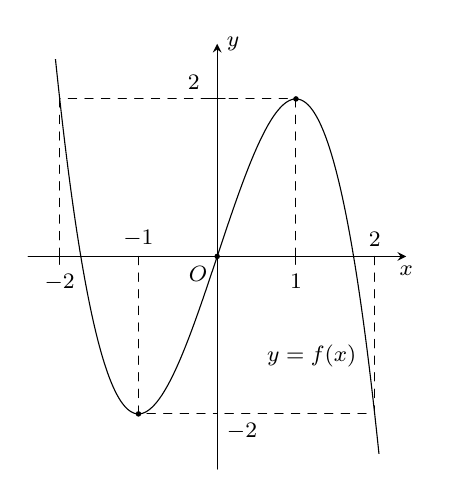
\begin{tikzpicture}[scale=1, font=\footnotesize, line join=round, line cap=round, >=stealth]
			\def\xmin{-2.2}
			\def\xmax{2.2}
			\def\ymin{-2.5}
			\def\ymax{2.5}
			\draw[->] (\xmin-0.2,0)--(\xmax+0.2,0) node[below] {\footnotesize $x$};
			\draw[->] (0,\ymin-0.2)--(0,\ymax+0.2) node[right] {\footnotesize $y$};
			\draw (0,0) node [below left] {\footnotesize $O$};
			\foreach \x in {-2,1}\draw (\x,0.1)--(\x,-0.1) node [below] {\footnotesize $\x$};
			\foreach \y in {2}\draw (0.1,\y)--(-0.1,\y) node [above left] {\footnotesize $\y$};
			\clip (\xmin,\ymin) rectangle (\xmax,\ymax);
			\draw[smooth,samples=200,domain=\xmin:\xmax] plot (\x,{-1*((\x)^3)+0*((\x)^2)+3*(\x)+0});
			\draw[dashed] (0.0,0)--(0.0,0.0)--(0,0.0);\fill (0.0,0.0) circle (1pt);
			\draw[dashed] (-1.0,0)--(-1.0,-2.0)--(0,-2.0);\fill (-1.0,-2.0) circle (1pt);
			\draw[dashed] (1.0,0)--(1.0,2.0)--(0,2.0);\fill (1.0,2.0) circle (1pt);
			\draw[dashed] (-2,0)--(-2,2)--(0,2);
			\draw[dashed] (2,0)--(2,-2)--(0,-2);
			\draw (2,0) node[above]{$2$};\draw (0,-2) node[below right]{$-2$};
			\draw (1.2,-1) node [below] {\footnotesize $y=f(x)$};
			\draw (-1,0) node[above]{$-1$};
		\end{tikzpicture}
	}
	\loigiai{
		Ta có $2^{f^2(x)+f(x)-m}-16\cdot 2^{f^2(x)-f(x)-m}-4^{f(x)}+16<0 \Leftrightarrow (4^{f(x)}-16)(2^{f^2(x)-f(x)-m}-1)<0$.\\
		Từ đồ thị đã cho ta thấy $x \in (-1; 1) \Rightarrow -2<f(x)<2$nên $4^{f(x)}-16<0$ với mọi $x \in (-1; 1)$.\\
		Bất phương trình đã cho có nghiệm $x\in (-1;1)$ khi và chỉ khi bất phương trình $2^{f^2(x)-f(x)-m}-1>0$ có nghiệm $x\in (-1;1)$, điều này tương đương với bất phương trình $f^2(x)-f(x)-m>0$ có nghiệm $x\in (-1;1)$.\\
		Đặt $t=f(x)$, $t \in (-2; 2)$. Bất phương trình trên trở thành $t^2-t>m$.\\
		Xét hàm số $g(t)=t^2-t$ với $t \in (-2; 2)$ ta có bảng biến thiên
		\begin{center}
			
\begin{tikzpicture}
				\tkzTabInit[nocadre=false,lgt=1.2,espcl=2.5,deltacl=0.6] %phần bắt buộc
				{$t$/0.6,$g(t)$/2}
				{$-2$,$\frac{1}{2}$,$2$}
				\tkzTabVar{+/$6$,-/$-\dfrac{1}{4}$,+/$2$}
			\end{tikzpicture}
		\end{center}
		Từ bảng biến thiên ta thấy bất phương trình $t^2-t>m$ có nghiệm $t \in (-2; 2)$ khi và chỉ khi $m<6$.\\
		Vì $m$ là số nguyên thuộc đoạn $[0; 9]$ nên ta được $m\in \{0; 1; 2; 3; 4; 5\}$.
	}
\end{ex}
\begin{ex}
	Cho bất phương trình $ \left(3^{x^2 - x} - 9 \right )\left ( 2^{x^2} - m \right ) \leq 0 $. Tìm số giá trị nguyên của $ m $ để bất phương trình đã cho có đúng $ 5 $ nghiệm nguyên.
	\choice
	{$ 65022 $}
	{\True $ 65024 $}
	{$ 65021 $}
	{$ 65023 $}
	\loigiai{
		Ta thấy $ 3^{x^2-x} - 9 < 0 \Leftrightarrow x^2 - x - 2 < 0 \Leftrightarrow -1< x < 2  $.\\
		Do vậy, bài toán cần tìm $ m $ nguyênđể $ \heva{& x \leq - 1 \lor x \geq 2 \\ & m \geq 2^{x^2}} \quad (*) $ có đúng $ 5 $ nghiệm $ x $ nguyên.\\
		Ta có bảng biến thiên của hàm số $ f(x) = 2^{x^2} $
		\begin{center}
			\begin{tikzpicture}[scale=0.8, font=\footnotesize, line join=round, line cap=round,>=stealth,yscale=.8,xscale=1.3]
				\def\cot{7} % số nhãn chiều dài
				\def\hang{4} % số nhãn chiều cao
				\draw[shift={(-.5,.5)}] 
				(0,0) rectangle +(\cot+1,-\hang-1)
				(0,-1)--+(0:\cot+1) 	
				(1,0)--+(-90:\hang+1);
				\path 
				(0,0) node{$x$} 
				(1,0) node{$-\infty$}
				(3,0) node{$-1$}
				(5,0) node{$2$}
				(7,0) node{$+\infty$}										 	
				(0,-2) node{$f(x)$}
				(1,-1) node (dvcL) {$+\infty$}												
				(7,-1) node (dvcR) {$+\infty$}
				(2.8,-4) node (CT) {$2$}
				(5.2,-3) node (CT1) {$2^4$}
				;
				\draw[->] (dvcL)--(CT);	
				\draw[->] (CT1)--(dvcR);
				\fill[pattern=north east lines,pattern color=gray] (3,-.5) rectangle (5,-4.5);
				\draw (3,-.5)--(3,-4.5) (5,-.5)--(5,-4.5);
			\end{tikzpicture}
		\end{center}		
		Từ bảng biến thiên, ta thấy $ (*) $ có đúng $ 5 $ nghiệm nguyên là $ \{-3;-2;-1;2;3 \} $, khi đó ta được $ 2^9 \leq m < 2^{16} $.\\
		Vậy có $ 2^{16} - 2^9 = 65024 $ giá trị nguyên của tham số $ m $ thoả đề bài.
	}
\end{ex}

\begin{ex}
	Cho bất phương trình $\log_3 (x^2-x+2)+1 \geq \log_3 (x^2+x+m-3)$. Có bao nhiêu giá trị nguyên của tham số $m$ để bất phương trình đã cho có nghiệm đúng với mọi giá trị $x$ thuộc đoạn $[0;6]$?
	\choice
	{$3$}
	{$6$}
	{\True $4$}
	{$5$}
	\loigiai{
		Điều kiện xác định
		\begin{align*}
			& x^2+x+m-3 >0, \forall x \in [0;6] \\
			\Leftrightarrow~& m > -x^2-x+3, \forall x \in [0;6].   \quad \quad (*)
		\end{align*}
		Hàm số $h(x) = -x^2-x+3$ nghịch biến trên $[0;6]$ nên $(*) \Leftrightarrow m> h(0) \Leftrightarrow m >3. \quad \quad (1)$  \\
		Ta có
		\begin{align*}
			& \log_3 (x^2-x+2)+1 \geq \log_3 (x^2+x+m-3), \forall x \in [0;6] \\
			\Leftrightarrow~ & \log_3 3(x^2-x+2) \geq \log_3 (x^2+x+m-3), \forall x \in [0;6] \\
			\Leftrightarrow~ & 3(x^2-x+2) \geq x^2+x+m-3, \forall x \in [0;6] \\
			\Leftrightarrow~ & m \leq 2x^2-4x+9 , \forall x \in [0;6]. \quad \quad (**)
		\end{align*}
		Bảng biến thiên của hàm số $g(x) = 2x^2-4x+9$ trên $[0;6]$
		\begin{center}
			
\begin{tikzpicture}
				\tkzTabInit[nocadre=false,lgt=1.2,espcl=2.5,deltacl=0.6]
				{$x$ /0.6,$g(x)$ /2}
				{$0$,$1$,$6$}
				\tkzTabVar{+/$9$,-/$7$,+/$57$}
			\end{tikzpicture}
		\end{center}
		Từ bảng biến thiên suy ra $(**) \Leftrightarrow m \leq 7. \quad \quad (2)$ \\
		Từ (1), (2) và $m$ nguyên  suy ra $m \in \{4;5;6;7\}$.
	}
\end{ex}
\begin{ex}
	Tìm $m$ để bất phương trình $1+\log_5(x^2+1)\ge \log_5(mx^2+4x+m)$ thỏa mãn với mọi $x\in\mathbb{R}$.
	\choice
	{\True $2<m\le 3$}
	{$2<m<3$}
	{$-1<m\le 0$}
	{$-1<m<0$}
	\loigiai{
		Ta có
		{\allowdisplaybreaks
			\begin{eqnarray*}
				&&1+\log_5(x^2+1)\ge \log_5(mx^2+4x+m) \\
				&\Leftrightarrow & \log_5[5(x^2+1)]\ge \log_5(mx^2+4x+m)\\
				&\Leftrightarrow & \heva{&5(x^2+1)\ge mx^2+4x+m\\& mx^2+4x+m>0} \\
				&\Leftrightarrow & \heva{&(5-m)x^2-4x+5-m\ge 0 & (1)\\&  mx^2+4x+m>0& (2)}
		\end{eqnarray*}}
		\begin{itemize}
			\item $(1)$ đúng với mọi $x\in\mathbb{R}$ khi và chỉ khi $\heva{&5-m>0\\&\Delta'_1=4-(5-m)^2\le 0}\Leftrightarrow m\le 3$.
			\item $(2)$ đúng với mọi $x\in\mathbb{R}$ khi và chỉ khi $\heva{&m>0\\&\Delta'_2=4-m^2<0}\Leftrightarrow m>2$.
		\end{itemize}
		Vậy,bất phương trình đã cho thỏa mãn với mọi $x\in\mathbb{R}$ khi và chỉ khi $2<m\le 3$.
	}
\end{ex}
\begin{ex}
	Cho bất phương trình $\log_3(x^2+2x+2)+1>\log_3(x^2+6x+5+m)$. Có tất cả bao nhiêu giá trị nguyên của tham số $m$ để bất phương trình trên nghiệm đúng với mọi $x\in (1;3)$?
	\choice
	{\True $14$}
	{$16$}
	{vô số}
	{$15$}
	\loigiai{
		Ta có \allowdisplaybreaks
		\begin{eqnarray*}
			&&\log_3(x^2+2x+2)+1>\log_3(x^2+6x+5+m)\\
			&\Leftrightarrow&\log_3\left(3x^2+6x+6\right)>\log_3(x^2+6x+5+m)\\
			&\Leftrightarrow& \heva{& x^2+6x+5+m>0 \\ & 3x^2+6x+6>x^2+6x+5+m}\\
			&\Leftrightarrow&\heva{& m>-x^2-6x-5 \\ & m<2x^2+1.} \quad (*)
		\end{eqnarray*}
		Đặt $f(x)=-x^2-6x-5$, $g(x)=2x^2+1$ với $x\in (1;3)$.\\
		Khi đó, hệ $(*)$ tương đương với $\heva{& m>\max\limits_{(1;3)} f(x) \\ &  m<\min\limits_{(1;3)} g(x).}$\\
		Bảng biến thiên của hàm số $f(x)$ trên $(1;3)$
		\begin{center}
			
\begin{tikzpicture}
				\tkzTabInit[nocadre=false,lgt=1.2,espcl=2.5,deltacl=0.6]
				{$x$ /0.6,$f(x)$ /2}
				{$1$,$3$}
				\tkzTabVar{+/$-12$, -/$-32$}
			\end{tikzpicture}
		\end{center}
		Bảng biến thiên của hàm số $g(x)$ trên $(1;3)$
		\begin{center}
			
\begin{tikzpicture}
				\tkzTabInit[nocadre=false,lgt=1.2,espcl=2.5,deltacl=0.6]
				{$x$ /0.6,$g(x)$ /2}
				{$1$,$3$}
				\tkzTabVar{-/$3$, +/$19$}
			\end{tikzpicture}
		\end{center}		
		Bất phương trình ban đầu có nghiệm đúng với mọi $x\in (1;3)$ khi và chỉ khi $\heva{& m>-12 \\ & m<3.}$\\
		Vì $m$ nguyên nên $m\in \{-11;-10;-9;-8;-7;-6;-5;-4;-3;-2;-1;0;1;2\}$
	}
\end{ex}
\begin{ex}
	Tổng tất cả các nghiệm nguyên của bất phương trình $\log_9(x + 6) - \log_3\left(5 - \sqrt[4]{19 - x}\right) < 0$ là
	\choice
	{\True $-12$}
	{$-11$}
	{$0$}
	{$-9$}
	\loigiai{
		Ta có $\log_9(x + 6) - \log_3\left(5 - \sqrt[4]{19 - x}\right) < 0 \Leftrightarrow \dfrac{1}{2}\log_3(x + 6) < \log_3\left(5 - \sqrt[4]{19 - x}\right)$\\
		\phantom{Ta có $\log_9(x + 6) - \log_3\left(5 - \sqrt[4]{19 - x}\right) < 0$} $\Leftrightarrow \heva{&-6 < x \leq 19 \\ &\sqrt{x + 6} < 5 - \sqrt[4]{19 - x}}$\\
		Xét bất phương trình $\sqrt{x + 6} < 5 - \sqrt[4]{19 - x}$ với $-6 < x \leq 19$.\\
		Ta có $\sqrt{x + 6} < 5 - \sqrt[4]{19 - x} \Leftrightarrow \sqrt{x + 6} - 3 + \sqrt[4]{19 - x} - 2 < 0$\\
		\phantom{Ta có $\sqrt{x + 6} < 5 - \sqrt[4]{19 - x}$} $\Leftrightarrow \dfrac{x - 3}{\sqrt{x + 6} + 3} + \dfrac{3 - x}{\left(\sqrt[4]{19 - x} + 2\right)\left(\sqrt{19 - x} + 4\right)} < 0$\\
		\phantom{Ta có $\sqrt{x + 6} < 5 - \sqrt[4]{19 - x}$} $\Leftrightarrow (x - 3)\left[\dfrac{1}{\sqrt{x + 6} + 3} - \dfrac{1}{\left(\sqrt[4]{19 - x} + 2\right)\left(\sqrt{19 - x} + 4\right)}\right] < 0$\\
		\phantom{Ta có $\sqrt{x + 6} < 5 - \sqrt[4]{19 - x}$} $\Leftrightarrow x < 3$\\ $\left(\mbox{Vì}\, \dfrac{1}{\sqrt{x + 6} + 3} - \dfrac{1}{\left(\sqrt[4]{19 - x} + 2\right)\left(\sqrt{19 - x} + 4\right)} \geq 0,\forall x \in (-6; 19]\right)$.\\
		Suy ra bất phương trình đã cho có tập nghiệm $S = (-6; 3)$.\\
		Vậy tổng tất cả các nghiệm nguyên của bất phương trình đã cho là
		\begin{center}
			$T = -5 + (-4) + (-3) + (-2) + (-1) + 0 + 1 + 2 = -12.$
		\end{center}
	}
\end{ex}
\begin{ex}
	Cho $x$, $y$ là các số thực dương thỏa mãn $\ln x+\ln y\ge \ln (x^2+y)$. Tìm giá trị nhỏ nhất của $P=x+y$.
	\choice
	{$P=2+3\sqrt{2}$}
	{$P=\sqrt{17}+\sqrt{3}$}
	{$P=6$}
	{\True $P=3+2\sqrt{2}$}
	\loigiai{
		Ta có $\ln x+\ln y\ge \ln (x^2+y)\Leftrightarrow xy\ge x^2+y\Leftrightarrow y(x-1)\ge x^2>0$.\\
		Suy ra $x>1$ và $y>0$.\\
		Khi đó $y\ge \dfrac{x^2}{x-1}$.\\
		Suy ra $P=x+y\ge x+\dfrac{x^2}{x-1}=2(x-1)+\dfrac{1}{x-1}+3\ge 2\sqrt{2(x-1)\cdot \dfrac{1}{x-1}}+3=2\sqrt{2}+3$.\\
		Vậy giá trị nhỏ nhất của biểu thức $P$ là $3+2\sqrt{2}$.
	}
\end{ex}

\begin{ex}
	Cho phương trình $\left(2\log_3^{2}x-\log_3x-1 \right)\sqrt{3^x-m}=0$ ($m$ là tham số thực). Có tất cả bao nhiêu giá trị nguyên dương của $m$ để phương trình đã cho có đúng hai nghiệm phân biệt.
	\choice
	{\True $26$}
	{$25$}
	{Vô số}
	{$24$}
	\loigiai
	{Điều kiện $\heva{&x>0\\&3^x-m\geq 0}$. Khi đó phương trình tương đương $\hoac{&\log_3{x}=1\\&\log_3{x}=-\dfrac{1}{2}\\&3^x=m} \Leftrightarrow \hoac{&x=3\\&x=\dfrac{1}{\sqrt{3}}\\&3^x=m.}$\\
		Vì $m$ là số nguyên dương nên ta xét các trường hợp sau:
		\begin{itemize}
			\item Trường hợp $1$: Với $m=1$, phương trình có hai nghiệm phân biệt $x=3$, $x=\dfrac{1}{\sqrt{3}}$.
			\item Trường hợp $2$: Với $m>1$, khi đó phương trình $3^x=m$ luôn có nghiệm dương $x=\log_3{m}$. Do đó phương trình đã cho có đúng hai nghiệm phận biệt khi và chỉ khi
			$$\dfrac{1}{\sqrt{3}}\leq \log_3{m}<3 \Leftrightarrow 3^{\tfrac{1}{\sqrt{3}}} \leq m <27.$$
		\end{itemize}
		Do $m$ nguyên dương nên phương trình đã cho có đúng hai nghiệm phân biệt khi và chỉ khi $m\in \{1;2;\ldots;26\}$. Vậy có $26$ giá trị của $m$ thỏa mãn yêu cầu bài toán.
	}
\end{ex}
\begin{ex}
	Cho $x\geq 0, y\geq 0, x+y>0$ thỏa mãn $2^{x^2+y^2}+2023^{x+y} \cdot \log _2 \dfrac{x^2+y^2}{x+y} \leq 4^{x+y}+2023^{x+y}$. Tìm tổng giá trị lớn nhất và giá trị nhỏ nhất của biểu thức $P=x^2+y^2-8x-2y+10$.
	\choice
	{$8$}
	{$12$}
	{$4+6\sqrt 2$}
	{\True $14-6\sqrt 2$}
	\loigiai{
		$$
		\begin{aligned}
			& 2^{x^2+y^2}+2023^{x+y} \cdot \log _2 \dfrac{x^2+y^2}{x+y} \leqslant 4^{x+y}+2023^{x+y}  \\
			& \Leftrightarrow 2^{x^2+y^2}+2023^{x+y} \cdot \log _2 \dfrac{x^2+y^2}{2(x+y)} \leq 4^{x+y}  \\
			& \Leftrightarrow 2023^{x+y} \cdot\left[\log _2\left(x^2+y^2\right)-\log _2[2(x+y)]\right] \leq 2^{2(x+y)}-2^{x^2+y^2}
		\end{aligned}
		$$
		Nếu $x^2+y^2>2(x+y)$. Khi đó $VT>0 ; VP<0$ (không thoả mãn).\\
		Nếu $x^2+y^2 \leq 2(x+y)$. Khi đó $VT \leq 0 ; VP \geq 0$ luôn thoả mãn.\\
		Vậy $x^2+y^2-2 x-2 y \leq 0 \Rightarrow(x;y)$ thuộc phần hình tròn tâm $I(1;1)$ bán kính $r=\sqrt{2}$ (với $x\geq0, y\geq 0, x+y>0$).\\
		Khi đó
		$P=x^2+y^2-8x-2y+10 \Rightarrow(x;y)$ thuộc phần đường tròn tâm $K(4;1)$ bán kính $R=\sqrt{P+7}$ thoả mãn $x\geq 0, y\geq 0, x+y>0; \mathrm{d}=KI=3$.
		\begin{center}
			\begin{tikzpicture}[x=1cm,y=1cm,scale=1]
				\draw[->] (-1,0)--(7,0)node[below right]{$x$};
				\draw[->] (0,-2)--(0,4)node[left]{$y$};
				\fill (0,0)node[below left]{ $O$};
				\path (1,0)coordinate[label=below:$1$](A) (2,0)coordinate[label=below:$2$](B) (3,0)coordinate[label=below:$3$](C) (4,0)coordinate[label=below:$4$](D) (5,0)coordinate[label=below:$5$](E) (6,0)coordinate[label=below:$6$](F) (0,-1)coordinate[label=left:$-1$](G) (0,1)coordinate[label=left:$1$](H) (0,2)coordinate[label=left:$2$](N) (0,3)coordinate[label=left:$3$](M) (1,1)coordinate[label=above:$I$](I) (4,1)coordinate[label=above:$K$](K) (1.8,0)coordinate(T);
				\draw[black] let \p1=($(N)-(I)$) in (I) circle ({veclen(\x1,\y1)});
				\draw[black] let \p1=($(T)-(K)$) in (K) circle ({veclen(\x1,\y1)});
				\coordinate (W) at ($(I)!1!45:(B)$);
				
				\draw[dashed] (W)--(K)--(N);
				
				\foreach \diem in {A,B,C,D,E,F,G,H,M,N,I,K,W} \fill[black](\diem)circle(1.5pt);
				
			\end{tikzpicture}
		\end{center}		
		Dựa vào hình vẽ, để tồn tại $(x;y)$ ta phải có $\mathrm{d}-r\leq R\leq KA,(A(0;2)) \Leftrightarrow 3-\sqrt{2} \leq \sqrt{P+7} \leq \sqrt{17}$
		$$
		\begin{aligned}
			& 11-6\sqrt 2\leq P+7\leq 17\Leftrightarrow 4-6\sqrt 2\leq P\leq 10\\ &	 P _{\max}+P _{\min}=10+4-6\sqrt 2=14-6\sqrt 2.
		\end{aligned}
		$$		
	}
\end{ex}
\Closesolutionfile{ans}
\begin{indapan}{10}
	{ANS/ans-1-6-4-5}
\end{indapan}
\begin{dang}{Bài toán thực tế, liên môn}
	
\end{dang}
\subsubsection{Ví dụ minh hoạ}

\begin{vd} 
	Dân số được ước tính theo công thức $S=A\cdot \mathrm{e}^{rt}$, trong đó $A$ là dân số của năm lấy làm mốc tính, $S$ là số dân sau $t$ năm, $r$ là tỉ lệ tăng dân số hằng năm. Giả sử $r=1{,}14\%$/năm, hỏi sau bao nhiêu năm dân số sẽ gấp đôi dân số ban đầu?
	\loigiai{
		Gọi $A$ là dân số ban đầu. Phương trình thể hiện dân số sau $t$ năm gấp đôi dân số ban đầu là
		\[
		A\cdot \mathrm{e}^{{0{,}0114}\cdot t}=2A \Leftrightarrow \mathrm{e}^{{0{,}0114}\cdot t} = 2 \Leftrightarrow 
		0{,}0114\cdot t = \ln 2 \Leftrightarrow t = \dfrac{\ln 2}{0{,}0114} \approx 61.
		\]
		Vậy sau $61$ năm dân số sẽ gấp đôi dân số ban đầu.
	}
\end{vd}

\begin{vd} 
	Chỉ số hay độ pH của một dung dịch được tính theo công thức: $\text{pH} = -\log [H^+]$ (trong đó $[H^+]$ chỉ nồng độ ion hydrogen). Đo chỉ số pH của một mẫu nước sông, ta có kết quả là $\text{pH} =6{,}1$. Hỏi nồng độ của ion hydrogen $[H^+]$ trong mẫu nước sông đó bằng bao nhiêu?
	\loigiai{
		Phương trình thể hiện nồng độ $x$ của ion hydrogen $[H^+]$ trong mẫu nước sông đó là
		\[
		-\log x=6{,}1 \Leftrightarrow \log x=-6{,}1 \Leftrightarrow x=10^{-6{,}1}
		\]
		Vậy nồng độ của ion hydrogen $[H^+]$ trong mẫu nước sông đó là $10^{-6{,}1}$ (mol L$^{-1}$).
	}
\end{vd}

\begin{vd} 
	Giả sử giá trị còn lại (tính theo triệu đồng) của một chiếc ô tô sau $t$ năm sử dụng được mô hình hóa bằng công thức
	$$V(t)=780\cdot (0{,}905)^t.$$
	Hỏi nếu theo mô hình này, sau bao nhiêu năm sử dụng thì giá trị của chiếc xe đó còn lại không quá $300$ triệu đồng? (Làm tròn kết quả đến hàng đơn vị).
	\loigiai{
		Giá trị còn lại của chiếc ô tô không quá $300$ triệu đồng khi và chỉ khi
		\[V(t)\leq 300\Leftrightarrow 780\cdot (0{,}905)^t\leq 300\Leftrightarrow (0{,}905)^t\leq \dfrac{5}{13}\Leftrightarrow t\geq \log_{0{,}905}\dfrac{5}{13}\approx 9{,}57.\]
		Vậy sau $10$ năm thì giá trị còn lại của chiếc ô tô không quá $300$ triệu đồng.
	}
\end{vd}

\begin{vd} 
	Nếu khối lượng carbon-$14$ trong cơ thể sinh vật lúc chết là $M_0(\mathrm{~g})$ thì khối lượng carbon-$14$ còn lại (tính theo gam) sau $t$ năm được tính theo công thức $M(t)=M_0\left(\dfrac{1}{2}\right)^{\tfrac{t}{T}}(\mathrm{~g})$, trong đó $T=5730$ (năm) là chu kì bán rã của carbon-$14$. Nghiên cứu hoá thạch của một sinh vật, người ta xác định được khối lượng carbon-$14$ hiện có trong hoá thạch là $5 \cdot 10^{-13} \mathrm{~g}$. Nhờ biết tỉ lệ khối lượng của carbon-$14$ so với carbon-$12$ trong cơ thể sinh vật sống, người ta xác định được khối lượng carbon-$14$ trong cơ thể lúc sinh vật chết là $M_0=1{,}2\cdot 10^{-12}(\mathrm{~g})$. Sinh vật này sống cách đây bao nhiêu năm? (Làm tròn kết quả đến hàng trăm.)
	\loigiai{
		Gọi $t$ là thời gian từ lúc sinh vật chết đến nay. Ta có:
		$$
		\begin{aligned}
			5\cdot 10^{-13}=1{,}2\cdot 10^{-12} \cdot\left(\dfrac{1}{2}\right)^{\tfrac{t}{T}} & \Leftrightarrow\left(\dfrac{1}{2}\right)^{\tfrac{t}{T}}=\dfrac{5}{12} \Leftrightarrow \dfrac{t}{T}=\log _{\tfrac{1}{2}} \dfrac{5}{12} \\
			& \Leftrightarrow t=T \log _{\tfrac{1}{2}} \dfrac{5}{12}=-5730 \cdot \log _2 \dfrac{5}{12} \approx 7237 \approx 7200.
		\end{aligned}
		$$
		Vậy sinh vật này sống cách đây khoảng $7200$ năm.
	}
\end{vd}

\begin{vd} 
	Công thức tính khối lượng còn lại của một chất phóng xạ từ khối lượng ban đầu $M_0$ là $M(t)=M_0\left(\dfrac{1}{2}\right)^{\tfrac{1}{T}}$, trong đó $t$ là thời gian tính từ thời điểm ban đầu và $T$ là chu kì bán rã của chất. Đồng vị plutonium-$234$ có chu kì bán rã là $9$ giờ.
	\begin{flushright}
		(\textit{Nguồn: https://pubchem.ncbi.nlm.nih.gov/element/Plutonium\#section=AtomicMass\\-Half-Life-and-Deca})
	\end{flushright}
	Từ khối lượng ban đầu $200 \mathrm{~g}$, sau bao lâu thì khối lượng plutonium-$234$ còn lại là
	\begin{listEX}[3]
		\item $100 \mathrm{~g}$?
		\item $50 \mathrm{~g}$?
		\item $20 \mathrm{~g}$?
	\end{listEX}
	\loigiai{
		\begin{listEX}
			\item $100 =200\left(\dfrac{1}{2}\right)^{\tfrac{t}{9}}\Leftrightarrow t=9$ giờ.
			\item $50=200\left(\dfrac{1}{2}\right)^{\tfrac{t}{9}}\Leftrightarrow t=18$ giờ.
			\item $20=200\left(\dfrac{1}{2}\right)^{\tfrac{t}{9}}\Leftrightarrow t=9\cdot \log_{\tfrac{1}{2}} \dfrac{1}{10} \approx 29{,}9$ giờ.
		\end{listEX}	
	}
\end{vd}

\begin{vd} 
	Nước chanh có độ pH bằng $2{,}4$; giấm có độ pH bằng $3$. Nước chanh có độ acid gấp bao nhiêu lần giấm (nghĩa là có nồng độ H$^{+}$ gấp bao nhiêu lần)? (Làm tròn kết quả đến hàng phần trăm).
	\loigiai{
		Kí hiệu $x, y$ lần lượt là nồng độ H$^{+}$ trong nước chanh và giấm.\\ Theo giả thiết, ta có $2{,}4=-\log x$ và $3=-\log y$.\\
		Suy ra $x=10^{-2{,}4}$ và $y=10^{-3}$. Suy ra $\dfrac{x}{y}=\dfrac{10^{-2{,}4}}{10^{-3}}=10^{0{,}6} \approx 3{,}98$.\\
		Vậy nồng độ H$^{+}$ của nước chanh gấp $3{,}98$ lần nồng độ H$^{+}$ của giấm.
	}
\end{vd}

\subsubsection{Bài tập rèn luyện} 

\begin{bt}
	Một người gửi ngân hàng $100$ triệu đồng theo hình thức lãi kép có kì hạn là $12$ tháng với lãi suất là $x$ $\%$/năm ($x>0$). Sau $3$ năm, người đó rút được cả gốc và lãi là $119{,}1016$ triệu đồng. Tìm $x$, biết rằng lãi suất không thay đổi qua các năm và người đó không rút tiền ra trong suốt thời gian gửi.
	\loigiai{
		Gọi $P_n$ là số tiền gốc và lãi nhận được sau $n$ kì gửi.\\
		$P_0$ là số tiền gửi ban đầu.\\
		$x\%$ lãi suất.\\
		Với $n=3$ năm, $P_3=119{,}1016$ triệu; $P_0=100$ triệu, ta có 
		\[
		P_3=P_0(1+x)^3 \Leftrightarrow (1+x)^3=\dfrac{P_3}{P_0} \Leftrightarrow
		1+x=\sqrt[3]{\dfrac{P_3}{P_0}} \]
		\[\Leftrightarrow x=\sqrt[3]{\dfrac{P_3}{P_0}}-1
		= \sqrt[3]{\dfrac{119{,}1016}{100}}-1=\dfrac{3}{50}=0{,}06=6\%
		\]
		Vậy lãi suất gửi là $6\%$/năm
	}
\end{bt}

\begin{bt}
	Sử dụng công thức tính mức cường độ âm $L$ ở ví dụ $14$, hãy tính mức cường độ âm mà tai người có thể nghe được, biết rằng tai nguời có thể nghe được âm với cường độ âm từ $10^{-12}$ W/m$^2$ đến $10$ W/m$^2$.
	\loigiai{
		Ta có công thức mức cường độ âm $L=10\log \dfrac{I}{10^{-12}}$, trong đó $I$ (đơn vị: W/m$^2$) là cường độ âm.\\
		Mức cường độ âm mà tai người có thể nghe được là
		\[
		10\log \dfrac{10^{-12}}{10^{-12}}<L<10\log \dfrac{10}{10^{-12}}
		\Leftrightarrow 0<L<130.
		\]
		Vậy mức cường độ âm mà tai người nghe được từ $0$ đến $130$ dB.
	}
\end{bt}

\begin{bt}
	Bác Minh gửi tiết kiệm $500$ triệu đồng ở một ngân hàng với lãi suất không đổi $7{,}5 \%$ một năm theo thể thức lãi kép kì hạn $12$ tháng. Tổng số tiền bác Minh thu được (cả vốn lẫn lãi) sau $n$ năm là:
	$$A=500 \cdot(1+0{,}075)^n \text { (triệu đồng).}$$
	Tính thời gian tối thiểu gửi tiết kiệm để bác Minh thu được ít nhất $800$ triệu đồng (cả vốn lẫn lãi).
	\loigiai{
		Ta cần tìm $n$ sao cho $$A\geq 800\Leftrightarrow 500\cdot (1+0{,}075)^n\geq 800\Leftrightarrow (1{,}075)^n\geq \dfrac{8}{5}\Leftrightarrow n\geq \log_{1{,}075}{\dfrac{8}{5}}\approx 6{,}5.$$
		Vậy sau khoảng $6{,}5$ năm gửi tiết kiệm, bác Minh thu được ít nhất $800$ triệu đồng.		
	}
\end{bt}	

\begin{bt}
	Số lượng vi khuẩn ban đầu trong một mẻ nuôi cấy là $500$ con. Người ta lấy một mẫu vi khuẩn trong mẻ nuôi cấy đó, đếm số lượng vi khuẩn và thấy rằng tỉ lệ tăng trưởng vi khuẩn là $40 \%$ mỗi giờ. Khi đó số lượng vi khuẩn $N(t)$ sau $t$ giờ nuôi cấy được ước tính bằng công thức sau:
	$$N(t)=500\mathrm{e}^{0{,}4t}.$$
	Hỏi sau bao nhiêu giờ nuôi cấy, số lượng vi khuẩn vượt mức $80000$ con?
	\loigiai{
		Kể từ lúc bắt đầu nuôi cấy, số lượng vi khuẩn vượt mức $80000$ con ta có
		$$500\mathrm{e}^{0{,}4t}\geq 80000\Leftrightarrow \mathrm{e}^{0{,}4t}\geq 160\Leftrightarrow 0{,}4t\geq \ln 160\Leftrightarrow t\geq\dfrac{\ln 160}{0{,}4}\approx 13\text{ (giờ)}.$$
		Vậy sau khoảng $13$ giờ nuôi cấy, số lượng vi khuẩn vượt mức $80000$ con.
	}
\end{bt}

\begin{bt}
	Giả sử nhiệt độ T ($^{\circ}$C) của một vật giảm dần theo thời gian cho bởi công thức:
	$$T=25+70\mathrm{e}^{-0{,}5t},$$ trong đó thời gian $t$ được tính bằng phút.
	\begin{enumerate}
		\item Tìm nhiệt độ ban đầu của vật.
		\item Sau bao lâu nhiệt độ của vật còn lại $30^{\circ}$C?
	\end{enumerate}
	\loigiai{
		\begin{enumerate}
			\item Nhiệt độ ban đầu của vật là $T_{0}=25+70\mathrm{e}^{-0{,}5\cdot0}=95$ ($^{\circ}$C).
			\item Nhiệt độ của vật còn lại 
			$30$ $^{\circ}$C, ta có 
			\begin{align*}
				30=25+70\mathrm{e}^{-0{,}5t} & \Leftrightarrow 70\mathrm{e}^{-0{,}5t}=5\Leftrightarrow \mathrm{e}^{-0{,}5t}=\dfrac{1}{14} \\
				&\Leftrightarrow -0{,}5t=\ln \dfrac{1}{14}\Leftrightarrow t\approx 5{,}3 \text{ (phút).}
			\end{align*}
		\end{enumerate}
	}
\end{bt}

\begin{bt}
	Tính nồng độ ion hydrogen (tính bằng mol/lít) của một dung dịch có độ pH là $8$.
	\loigiai{
		Nồng độ ion hydrogen trong dung dịch đó là $\left[H^{+}\right]=10^{-8}$.
	}
\end{bt}

\begin{bt}
	Chất phóng xạ polonium-$210$ có chu kì bán rã là $138$ ngày. Điều này có nghĩa là cứ sau 138 ngày, lượng polonium còn lại trong một mẫu chỉ bằng một nửa lượng ban đầu. Một mẫu $100 \mathrm{~g}$ có khối lượng polonium-$210$ còn lại sau $t$ ngày được tính theo công thức $M(t)=100\left(\dfrac{1}{2}\right)^{\tfrac{t}{138}}(\mathrm{~g})$.
	\begin{flushright}
		(Nguồn:https://pubchem.ncbi.nlm.nih.gov/element/Polonium\#section=\\
		Atomic-Mass-Half-Life-and-Decay)
	\end{flushright}
	\begin{itemize}
		\item[a)] Khối lượng polonium-$210$ còn lại bao nhiêu sau $2$ năm?
		\item[b)] Sau bao lâu thì còn lại $40 \mathrm{~g}$ polonium-$210$?
	\end{itemize}
	\loigiai{
		\begin{itemize}
			\item[a)] Đổi $2$ năm = $730$ ngày.\\
			Khối lượng polonium-$210$ còn lại sau $2$ năm là
			$$M(t)=100\left(\dfrac{1}{2}\right)^{\tfrac{730}{138}}\approx 2{,}556\mathrm{~g}.$$
			\item[b)] $100\left(\dfrac{1}{2}\right)^{\tfrac{t}{138}}=40\Leftrightarrow \left(\dfrac{1}{2}\right)^{\tfrac{t}{138}}=\dfrac{2}{5}\Leftrightarrow t=138\cdot \log_{\tfrac{1}{2}} \dfrac{2}{5}\approx 182{,}4$.\\
			Vậy cần $185$ ngày để còn lại $40 \mathrm{~g}$ polonium-$210$.
		\end{itemize}
	}
\end{bt}
\begin{bt}
	Nhắc lại rằng, mức cường độ âm $L$ được tính bằng công thức $L=10 \log \left(\dfrac{I}{I_0}\right)(\mathrm{dB})$, trong đó $I$ là cường độ của âm tính bằng $\mathrm{W}/ \mathrm{m}^2$ và $I_0=10^{-12} \mathrm{~W} / \mathrm{m}^2$.
	\begin{flushright}
		(Nguồn: Vật lí 12, NXB Giáo dục Việt Nam, năm 2017, trang 52)
	\end{flushright}
	\begin{itemize}
		\item[a)] Một giáo viên đang giảng bài trong lớp học có mức cường độ âm là $50 \mathrm{~dB}$. Cường độ âm của giọng nói giáo viên bằng bao nhiêu?
		\item[b)] Mức cường độ âm trong một nhà xưởng thay đổi trong khoảng từ $75 \mathrm{~dB}$ đến $90 \mathrm{~dB}$. Cường độ âm trong nhà xưởng này thay đổi trong khoảng nào?
	\end{itemize}
	\loigiai{
		\begin{itemize}
			\item[a)] Ta có $L=50\Leftrightarrow 10\log \left(\dfrac{I}{I_0}\right)=50\Leftrightarrow \log \left(\dfrac{I}{I_0}\right)=5\Leftrightarrow I=T_0\cdot 10^5\Leftrightarrow I=10^{-7} \mathrm{~W}/\mathrm{m}^2$.\\
			Vậy cường độ âm của giọng nói giáo viên bằng $10^{-7} \mathrm{~W}/\mathrm{m}^2$.
			\item[b)] Ta có $75<L<90\Leftrightarrow 7{,}5<\log \left(\dfrac{I}{I_0}\right)<9\Leftrightarrow 10^{-2{,}5}<I<10^{-3}$.\\
			Vậy cường độ âm trong nhà xưởng này thay đổi trong khoảng từ $10^{-2{,}5}\mathrm{~W}/\mathrm{m}^2$ đến $10^{-3}\mathrm{~W}/\mathrm{m}^2$.
		\end{itemize}
	}
\end{bt}
\subsubsection{Bài tập trắc nghiệm}
\Opensolutionfile{ans}[ANS/ans-1-6-4-6]
\begin{ex}
	Ông $A$ gửi $100$ triệu đồng vào ngân hàng theo thể thức lãi kép kì hạn một năm với lãi suất là $12\%$ một năm. Sau $n$ năm ông $A$ rút toàn bộ tiền (cả vốn lẫn lãi). Tìm $n$ nguyên dương nhỏ nhất để số tiền lãi nhận được hơn $40$ triệu đồng. (Giả sử rằng lãi suất hàng năm không thay đổi).
	\choice
	{$5$}
	{\True $3$}
	{$2$}
	{$4$}
	\loigiai{
		Số tiền lãi sau $n$ năm là $100(1+12\%)^n-100$ (triệu đồng).\\
		Ta có $100(1+12\%)^n-100>40\Leftrightarrow 1{,}12^n>\dfrac{7}{5}\Rightarrow n>2{,}96$.\\
		Vậy giá trị nguyên dương nhỏ nhất của $n$ là $3$.
	}
\end{ex}
\begin{ex}
	Anh A vào làm ở công ty X với mức lương ban đầu là $10$ triệu đồng/ tháng. Nếu hoàn thành tốt nhiệm vụ thì cứ sau $6$ tháng làm việc, mức lương của anh lại được tăng thêm 20\%. Hỏi bắt đầu từ tháng thứ mấy kể từ khi vào làm ở công ty X, tiền lương mỗi tháng của anh A nhiều hơn $20$ triệu đồng(biết rằng trong suốt thời gian làm ở công ty X anh A luôn hoàn thành tốt nhiệm vụ?
	\choice
	{Tháng thứ $31$}
	{Tháng thứ $19$}
	{Tháng thứ $37$}
	{\True Tháng thứ $25$}
	\loigiai{
		Tiền lương mỗi tháng lúc ban đầu là $a=10$.\\
		Sau chu kì mỗi lần $6$ tháng hoàn thành tốt nhiệm vụ, mức lương tăng thêm là $r=20\%$.
		Áp dụng công thức lãi suất kép, ta có mức lương mỗi tháng sau $n$ kì hạn (mỗi kì hạn $6$ tháng)
		$$\mathrm{P}_n=a(1+r)^n.$$
		Bài toán đưa về việc tìm số tự nhiên $k$ nhỏ nhất sao cho $$\mathrm{P}_k>20 \Leftrightarrow a(1+r)^k>20 \Leftrightarrow (1+r)^k>2 \Leftrightarrow k>\log_{1+r}2 \Leftrightarrow k>3,8 \Rightarrow k=4.$$
		Vậy sau $1$ tháng lương đầu tiên và $4$ kì hạn tiếp theo (mỗi kì hạn $6$ tháng), anh A sẽ nhận được mức lương nhiều hơn $20$ triệu đồng mỗi tháng.}
\end{ex}
\begin{ex}
	Đầu năm $2018$, ông An thành lập một công ty sản xuất rau sạch. Tổng số tiền ông An dùng để trả lương
	cho nhân viên trong năm $2018$ là $1$ tỷ đồng. Biết rằng cứ sau mỗi năm thì tổng số tiền dùng để trả lương cho nhân
	viên trong cả năm tăng thêm $15\%$ so với năm trước. Năm đầu tiên ông An phải trả lương cho nhân viên trong cả
	năm vượt qua $2$ tỷ đồng là năm nào?
	\choice
	{Năm $2020$}
	{Năm $2025$}
	{Năm $2022$}
	{\True Năm $2023$}
	\loigiai{
		Số tiền ông An trả lương cho nhân viên trong năm thứ $n$ là $T_n=1 \cdot \left( 1+\dfrac{15}{100} \right)^n$.\\
		$$T_n > 2 \Leftrightarrow  \left( 1+\dfrac{15}{100} \right)^n > 2 \Leftrightarrow n > 4{,} 95.$$
		Vậy sau $5$ năm hay năm $2023$ thì số tiền ông An trả lương cho nhân viên vượt qua $2$ tỷ.
	}
\end{ex}
\begin{ex}
	Một người gửi vào ngân hàng số tiền $30$ triệu đồng, lãi suất $0{,}48\%$ /tháng. Sau đúng $1$ tháng kể từ ngày gửi người này gửi đều đặn thêm vào $1$ triệu đồng, hai lần gửi liên tiếp cách nhau đúng $1$ tháng. Giả định rằng lãi suất không thay đổi và người này không rút tiền ra, số tiền lãi của tháng trước được tính vào vốn và tính lãi cho tháng kế tiếp. Hỏi sau ít nhất bao nhiêu tháng người này thu về tổng số tiền cả gốc và lãi ít nhất $50$ triệu đồng.
	\choice
	{$19$}
	{$20$}
	{$17$}
	{\True $18$}
	\loigiai{
		Đặt $r=0{,}48\%=0{,}0048$.\\
		Tổng số tiền người này nhận được sau đúng $n$ tháng kể từ ngày gửi là
		\begin{eqnarray*}
			A_n&=&30(1+r)^n+(1+r)^{n-1}+(1+r)^{n-2}+ \cdots +(1+r)\\
			&=&30(1+r)^n+(1+r) \cdot \dfrac{(1+r)^{n-1}-1}{r}\\
			&=&(1+r)^n\left(30+\dfrac{1}{r}\right)-\dfrac{1+r}{r}.
		\end{eqnarray*}
		Yêu cầu bài toán
		\begin{eqnarray*}
			A_n \geq 50 &\Leftrightarrow& (1+r)^n\left(30+\dfrac{1}{r}\right)-\dfrac{1+r}{r} \geq 50\\
			& \Leftrightarrow & 1{,}0048^n \geq \dfrac{50+\dfrac{1{,}0048}{0,0048}}{30+\dfrac{1}{0{,}0048}}\\
			& \Leftrightarrow& n \geq \log_{1,0048}\dfrac{50+\dfrac{1{,}0048}{0{,}0048}}{30+\dfrac{1}{0{,}0048}}\\
			& \approx& 17{,}6.
		\end{eqnarray*}
		Vậy ít nhất sau $18$ tháng người này thu về số tiền ít nhất $50$ triệu đồng.}
	%<MyLT>
\end{ex}
\begin{ex}
	Ông A gửi vào ngân hàng $50$ triệu đồng với lãi suất $0{,}5\%$/tháng. Hỏi ít nhất bao nhiêu tháng thì ông A có số tiền cả gốc lẫn lãi nhiều hơn $60$ triệu đồng? Biết rằng trong suốt thời gian gửi lãi suất ngân hàng không thay đổi và ông A không rút tiền ra.
	\choice
	{\True $37$ tháng}
	{$38$ tháng}
	{$40$ tháng}
	{$36$ tháng}
	\loigiai{
		Số tiền ông Agửi sau $n$ tháng là $P_n = 50\cdot \left(1+0{,}5\%\right)^n$ \, (triệu đồng).\\
		Để số tiền ông A thu được nhiều hơn $60$ triệu đồng thì $$50\cdot \left(1+0{,}5\%\right)^n>60 \Leftrightarrow n > \log_{1+0{,}5\%}\dfrac{6}{5}\approx 36{,}555.$$
		Vậy ông $A$ phải gửi ít nhất là $37$ tháng.
	}
\end{ex}
\begin{ex}
	Đầu năm $2016$, ông A thành lập một công ty. Tổng số tiền ông A dùng để trả lương cho nhân viên trong năm $2016$ là $1$ tỷ đồng. Biết rằng cứ sau mỗi năm thì tổng số tiền để trả cho nhân viên trong cả năm đó tăng thêm $15\%$ so với năm trước. Hỏi năm nào dưới đây là năm đầu tiên mà tổng số tiền ông A dùng để trả lương cho nhân viên trong cả năm lớn hơn $2$ tỷ đồng?
	\choice
	{\True  Năm $2021$ }
	{Năm $2022$}
	{Năm $2023$}
	{Năm $2020$}
	\loigiai{
		Năm $2016$ là năm đầu tiên ông A trả lương cho nhân viên. Tổng số tiền phải trả là $T_0 = 1$ tỷ.\\
		Tổng số tiền ông A phải trả cho nhân viên ở năm thứ $n$ là $T_n= 1 \cdot \left(1+15\%\right)^n$.\\
		Theo đề bài ta có $T_n >2 \Leftrightarrow \left(1+15\%\right)^n >2 \Leftrightarrow n > \log_{\left(1+15\%\right)} 2 \approx 4{,}9$.\\
		Hay sau $5$ năm tức là năm $2021$, tổng số tiền ông A dùng để trả lương cho nhân viên trong cả năm lớn hơn $2$ tỷ đồng.
	}
\end{ex}
\begin{ex}
	Một người gửi tiền vào ngân hàng với lãi suất không thay đổi là $8\%/\text{năm}$. Biết rằng nếu không rút tiền ra khỏi ngân hàng thì cứ sau mỗi năm, số tiền lãi sẽ được nhập vào vốn ban đầu (người ta gọi là lãi suất kép). Người đó định gửi tiền trong vòng $3$ năm, sau đó rút tiền ra để mua một căn hộ chung cư trị giá $500$ triệu đồng. Hỏi số tiền ít nhất người đó phải gửi vào ngân hàng để có đủ tiền mua căn hộ chung cư (kết quả làm tròn đến hàng triệu) là bao nhiêu?
	\choice
	{$395$ triệu đồng}
	{$396$ triệu đồng}
	{\True $397$ triệu đồng}
	{$394$ triệu đồng}
	\loigiai{
		Gọi $A$ là số tiền gửi ban đầu.\\
		Theo công thức lãi kép, số tiền người đó nhận được sau $3$ năm là $T=A(1+r)^3$.\\
		Theo đề bài, ta cần có $T \geq 500 \Leftrightarrow A(1+r)^{3} \geq 500 \Leftrightarrow A \geq \dfrac{500}{(1+8 \%)^{3}} \approx 397$ triệu đồng.\\
		Vậy người đó phải gửi ít nhất $397$ triệu đồng.
	}
\end{ex}
\begin{ex}
	Anh Nam muốn mua một ngôi nhà trị giá $ 500 $ triệu đồng sau $ 3 $ năm nữa. Biết rằng lãi suất hàng năm vẫn không đổi là $ 8\% $ một năm. Vậy ngay từ bây giờ số tiền ít nhất anh Nam phải gửi tiết kiệm vào ngân hàng theo thể thức lãi kép để có đủ tiền mua nhà (kết quả làm tròn đến hàng triệu) là
	\choice
	{$ 395 $ triệu đồng}
	{\True $ 397 $ triệu đồng}
	{$ 394 $ triệu đồng}
	{$ 396 $ triệu đồng}
	\loigiai{
		Gọi $ x $ là số tiền anh Nam phải giải tiết kiệm, đơn vị triệu đồng. Khi đó sau 3 năm, theo hình thức lãi kép thì số tiền anh Nam nhận được là $ x\left(1+ \dfrac{8}{100} \right)^3 $. \
		Vậy ta cần tìm $ x $ là số nguyên nhỏ nhất thỏa mãn điều kiện
		\[ x\left(1+ \dfrac{8}{100} \right)^3 \ge 500 \Leftrightarrow x \ge \dfrac{500}{\left(1+ \dfrac{8}{100} \right)^3} \approx 396,9. \]
		Vậy $ x = 397 $ triệu đồng.
	}
\end{ex}
\begin{ex}
	Một người gửi $300$ triệu đồng vào ngân hàng theo thể thức lãi kép kì hạn một quý, với lãi suất $1{,}75 \%$/một quý. Hỏi sau ít nhất bao nhiêu tháng người gửi có ít nhất $500$ triệu đồng (bao gồm cả vốn lẫn lãi) từ số vốn ban đầu? (Giả sử lãi suất không thay đổi).
	\choice
	{$29$ tháng}
	{$87$ tháng}
	{$30$ tháng}
	{\True $90$ tháng}
	\loigiai{
		Đặt $r=1+1{,}75 \%=1{,0175}$.\\
		Sau quý thứ nhất, người đó có $300+300 \cdot 1{,}75 \% = 300r$.\\
		Sau quý thứ hai, người đó có $300r+300r \cdot 1{,}75 \% =300r^2$.\\
		$\ldots$\\
		Sau quý thứ $n$, người đó có $300r^n$.\\
		Ta có $300r^n \ge 500 \Leftrightarrow n \ge \log_r \dfrac{5}{3}$.\\
		Mà $n \in \mathbb{N}$ nên $n \ge 30$.\\
		Suy ra sau ít nhất $30$ quý, hay nói cách khác, sau ít nhất $90$ tháng, người đó có ít nhất $500$ triệu đồng.
	}
\end{ex}
\begin{ex}
	Để đủ tiền mua nhà, anh An vay ngân hàng $500$ triệu theo phương thức trả góp với lãi suất $0{,}85\%$ một tháng. Nếu sau mỗi tháng, kể từ thời điểm vay, anh An trả nợ cho ngân hàng số tiền cố định là $10$ triệu đồng bao gồm cả tiền lãi vay và tiền gốc. Biết phương thức trả lãi và gốc không thay đổi trong suốt quá trình anh An trả nợ. Hỏi sau bao nhiêu tháng thì anh trả hết nợ ngân hàng? (tháng cuối có thể trả dưới $10$ triệu đồng).
	\choice
	{\True $66$}
	{$67$}
	{$65$}
	{$68$}
	\loigiai{
		Đặt $N=500$; $A=10$; $r=0{,}85\%$.\\
		Sau một tháng anh An còn nợ: $N\cdot (1+r)-A$.\\
		Sau hai tháng anh An còn nợ\\
		$(N\cdot (1+r)-A)\cdot (1+r)-A=N\cdot (1+r)^2-A\cdot\left[(1+r)+1\right]=N\cdot(1+r)^2-\dfrac{A}{r}\left[(1+r)^2-1\right]$.\\
		Tương tự sau $n$ tháng anh An còn nợ $N\cdot(1+r)^n-\dfrac{A}{r}\left[(1+r)^n-1\right]$.\\
		Anh An trả hết nợ sau $n$ tháng khi $n$ là nghiệm nguyên dương nhỏ nhất của bất phương trình
		\begin{eqnarray*}
			&N\cdot (1+r)^n-\dfrac{A}{r}\left[(1+r)^n-1\right]\leq 0&\Leftrightarrow 500\cdot (1+0{,}85\%)^n-\dfrac{10}{0{,}85\%}\left[(1+0{,}85\%)^n-1\right]\leq 0\\
			&&\Leftrightarrow (1+0{,}85\%)^n\geq\dfrac{40}{23}\\
			&&\Leftrightarrow n\geq \log_{1+0{,}85\%}\dfrac{40}{23}\approx 65{,}38.
		\end{eqnarray*}
		$\Rightarrow n=66$.
	}
\end{ex}
\begin{ex}
	Anh sinh viên A, sau khi ra trường, mong muốn rằng sau một năm sẽ có hơn $60$ triệu đồng để mua xe. Hàng tháng anh A phải gửi vào ngân hàng một số tiền như nhau là $m$. Hỏi $m$ nhỏ nhất là bao nhiêu?(làm tròn đến nghìn đồng). Biết rằng lãi suất ngân hàng là $0{,}6$ \%/tháng và hàng tháng số tiền lãi được nhập vào gốc.
	\choice
	{\True $4\ 809\ 000$ đồng}
	{$4\ 808\ 000$ đồng}
	{$4\ 890\ 000$ đồng}
	{$4\ 812\ 000$ đồng}
	\loigiai{
		Gọi $T_n$ là số tiền anh A có được sau $n$ tháng, $n \in \mathbb{N}$.\\
		Gọi $r (\%)$ là lãi suất của ngân hàng, $r>0$.\\
		Gọi $m$ là số tiền hàng tháng anh A gửi vào ngân hàng, $m$ không đổi, $m>0$.\\
		Đến cuối tháng thứ nhất, anh A có số tiền là $T_1=m+m \cdot r=m(1+r)$.\\
		Đến cuối tháng thứ hai, anh A có số tiền là
		\begin{eqnarray*}
			T_2 &=&(T_1+m)(1+r)\\& =&m(1+r)+m+[m(1+r)+m]r \\&=&m[(1+r)^2+(1+r)]\\
			&=&m\dfrac{(1+r)^3-(1+r)}{r}.
		\end{eqnarray*}
		Đến cuối tháng thứ ba, anh A có số tiền là $T_3=(T_2+m)(1+r)=m\dfrac{(1+r)^4-(1+r)}{r}$. \\
		Tổng quát, đến cuối tháng thứ $n$, anh A có số tiền là $T_n=m\dfrac{(1+r)^{n+1}-(1+r)}{r}$.\\
		Để sau $1$ năm, anh A có số tiền hơn $60$ triệu đồng thì phải có
		\allowdisplaybreaks
		\begin{eqnarray*}
			T_{12}=m\dfrac{(1+r)^{13}-(1+r)}{r}>60 \Leftrightarrow m>\dfrac{60 \cdot r}{(1+r)^{13}-(1+r)}=\dfrac{60 \cdot 0{,}6\%}{\left(1+0{,}6\%\right)^{13}-(1+0{,}6\%)} \approx 4{,}808300.
		\end{eqnarray*}
		Vậy anh A cần gửi vào ngân hàng mỗi tháng nhiều hơn $4\ 809\ 000$ đồng.
	}
\end{ex}
\begin{ex}
	Giả sử vào cuối năm thì một đơn vị tiền tệ mất $ 10\% $ giá trị so với đầu năm. Tìm số nguyên dương nhỏ nhất sao cho sau $ n $ năm, đơn vị tiền tệ sẽ mất đi ít nhất $ 90\% $ giá trị của nó?
	\choice
	{$ 20 $}
	{$ 16 $}
	{$ 18 $}
	{\True $ 22 $}
	\loigiai{
		Giả sử giá trị của đơn vị tiền tệ đang xét là $ A $. Ta thấy\\
		- Sau năm thứ $ 1 $: giá trị của đơn vị tiền tệ còn lại $ \dfrac{9}{10}A $.\\[5pt]
		- Sau năm thứ $ 2 $: giá trị của đơn vị tiền tệ còn lại $ \left (\dfrac{9}{10} \right )^2 A $.\\[5pt]
		- Sau năm thứ $ n $: giá trị của đơn vị tiền tệ còn lại $ \left (\dfrac{9}{10} \right )^n A $.\\
		Theo đề bài, ta cần tìm $ n $ nhỏ nhất sao cho $ \left (\dfrac{9}{10} \right )^n A < \dfrac{1}{10}A \Rightarrow n > 21{,}85 \Rightarrow n = 22 $.
	}
\end{ex}
\begin{ex}
	Ông A bị nhiễm một loại vi-rút nên phải nhập viện và được điều trị ngay lập tức. Kể từ ngày bắt đầu nhập viện, sau mỗi ngày điều trị thì lượng vi-rút trongg cơ thể ông A giảm đi $10\%$ so với ngày trước đó. Hỏi sau ít nhất bao nhiêu ngày thì ông A sẽ được xuất viện, biết ông được xuất viện khi lượng vi-rút trong cơ thể của ông không vượt quá $30\%$?
	\choice
	{$14$ ngày}
	{$11$ ngày}
	{\True $12$ ngày}
	{$13$ ngày}
	\loigiai{
		Gọi $x$ là số lượng vi khuẩn ban đầu.\\
		Số lượng vi khuẩn sau $n$ ngày là $x\left(1-10\%\right)^n$.\\
		Theo đề bài ta có $x(1-10\%)^n\le x\cdot 30\% \Leftrightarrow (1-10\%)^n\le 30\% \Leftrightarrow x\ge \log_{1-10\%}30\%\approx 11,42$.\\
		Vậy sau ít nhất $12$ ngày thì ông A được xuất viện.
	}
\end{ex}
\begin{ex}
	Một nghiên cứu cho thấy một nhóm học sinh được cho xem cùng một danh sách các loài sinh vật và được kiểm tra lại xem họ nhớ bao nhiêu phần trăm mỗi tháng. Sau $t$ tháng, khả năng nhớ trung bình của nhóm học sinh được cho bởi công thức $M(t)=60-15 \ln (t+1)$, $t>0$ (đơn vị phần trăm). Hỏi sau ít nhất bao nhiêu tháng thì nhóm học sinh chỉ nhớ được không vượt quá $10\%$ danh sách đó?
	\choice
	{\True $28$ tháng}
	{$27$ tháng}
	{$24$ tháng}
	{$25$ tháng}
	\loigiai{
		Xét bất phương trình
		\[
		\begin{aligned}
			M(t) \le 10\% &\Leftrightarrow 60 - 15\ln \left(t + 1\right)\le 10 \\
			&\Leftrightarrow 15\ln \left(t + 1\right)\ge 50 \\
			&\Leftrightarrow \ln \left(t + 1\right) \ge  \dfrac{10}{3}\\
			&\Leftrightarrow t  \ge \mathrm{e}^{\frac{10}{3}} - 1 \approx 27{,}03.
		\end{aligned}
		\]
		Vậy sau ít nhất $28$ tháng thì nhóm học sinh chỉ nhớ được không vượt quá $10\%$ danh sách đó.
	}
\end{ex}
\begin{ex}
	Bộ Y tế phát đi một thông tin tuyên truyền về phòng chống dịch COVID-19. Thông tin này lan truyền đến người dân theo công thức $P(t)=\dfrac{1}{1+a\mathrm{e}^{-kt}}$, với $P(t)$ là tỉ lệ dân số nhận được thông tin vào thời điểm $t$ và $a$, $k$ là các hằng số dương. Cho $a=3$, $k=\dfrac{1}{2}$ với $t$ đo bằng giờ. Hỏi cần phải ít nhất bao lâu để hơn 90\% dân số nhận được thông tin?
	\choice
	{$5{,}5$ giờ}
	{$8$ giờ}
	{$4{,}5$ giờ}
	{\True $6{,}6$ giờ}
	\loigiai{
		Cho $a=3$, $k=\dfrac{1}{2}$ thì $P(t)=\dfrac{1}{1+3\mathrm{e}^{-\tfrac{1}{2}t}}$ \\
		Với $P(t)\ge 90\%\Leftrightarrow \dfrac{1}{1+3\mathrm{e}^{-\tfrac{1}{2}t}}\ge \dfrac{90}{100}\Leftrightarrow t\ge -2\ln \dfrac{1}{27}\approx 6{,}6$ (giờ).\\
		Vậy cần ít nhất $6{,}6$ giờ để hơn 90\% dân số nhận được thông tin.
	}
\end{ex}

\begin{ex}
	Một nhóm các chuyên gia y tế đang nghiên cứu và thử nghiệm độ chính xác của một bộ xét nghiệm COVID-19. Giả sử cứ sau $n$ lần thử nghiệm và điều chỉnh bộ xét nghiệm thì tỉ lệ chính xác của bộ xét nghiệm đó tuân theo công thức $S(n)=\dfrac{1}{1+2020\cdot 10^{-0{,}01n}}$. Hỏi phải tiến hành ít nhất bao nhiêu lần thử nghiệm và điều chỉnh bộ xét nghiệm để đảm bảo tỉ lệ chính xác của bộ xét nghiệm đó đạt trên $90\%$?
	\choice
	{$428$}
	{$427$}
	{\True $426$}
	{$425$}
	\loigiai{
		Theo đề bài ta có
		\begin{eqnarray*}
			&& \dfrac{1}{1+2020\cdot 10^{-0{,}01n}}>90\%\\
			&\Leftrightarrow& 1+2020\cdot 10^{-0{,}01n}<\dfrac{1}{90\%}\\
			&\Leftrightarrow& 10^{-0{,}01n}< \dfrac{1}{18180}\\
			&\Leftrightarrow& -0{,}01n<\log \left(\dfrac{1}{18180}\right)\\
			&\Leftrightarrow& n>\dfrac{\log \left(\dfrac{1}{18180}\right)}{-0{,}01} \approx425{,}96.\\
		\end{eqnarray*}
		Vậy số lần xét nghiệm tối thiểu là $426$ lần.
	}
\end{ex}
%\Closesolutionfile{ans}
\begin{indapan}{10}
	{ANS/ans-1-6-4-6}
\end{indapan}